\documentclass{cumcm}


% \title{text}这里是显示在第三页的文章标题
\title{基于的目标规划模型的系泊系统设计}
% \displaytitle{text} 这里是显示在承诺书上的文章标题,注意,不能换行,如果题目特别长,要进行适当的缩写
\displaytitle{基于的目标规划模型的系泊系统设计}
% \school{text}命令用于在承诺书上显示学校名称。按要求,此处应填写全称
\school{上海交通大学}
% 以下命令分别显示队员、指导教师姓名以及队伍编号
\authorone{}
\authortwo{}
\authorthree{}
\advisor{}
\teamnumber{}

\begin{document}

% 这里用于打印承诺书以及编号页
 
%\newpage
\thispagestyle{empty} %取消当前页码
{\Large \heiti \begin{center}\the\year~高教社杯全国大学生数学建模竞赛\par\vspace{0.5\ccwd}\par
{\ziju{1}承诺书}\end{center}\par\vspace{1\ccwd}\par}
\renewcommand{\baselinestretch}{1.5}\normalsize
{\zihao{-4}%
我们仔细阅读了中国大学生数学建模竞赛的竞赛规则。\par
我们完全明白,在竞赛开始后参赛队员不能以任何方式(包括电话、电子邮件、网上咨询等)
与队外的任何人(包括指导教师)研究、讨论与赛题有关的问题。\par
我们知道,抄袭别人的成果是违反竞赛规则的, 如果引用别人的成果或其他公开的资料
(包括网上查到的资料),必须按照规定的参考文献的表述方式在正文引用处和参考文献中明确列出。\par
我们郑重承诺,严格遵守竞赛规则,以保证竞赛的公正、公平性。如有违反竞赛规则的行为,我们将受到严肃处理。\par
\par\vspace{2\ccwd}\par
\raisebox{1ex}[0pt]{我们参赛的题目是:}\vbox{\hbox to11.4cm{\hfil \the\displaytitle \hfil}
        \protect\vspace{0.6truemm}\relax
        \hrule depth0pt height0.15truemm width11.4cm}\par
\vspace{1mm}
\raisebox{1ex}[0pt]{我们的参赛报名号为(如果赛区设置报名号的话):}\vbox{\hbox to5.75cm{\hfil \the \teamnumber  \hfil}
        \protect\vspace{0.6truemm}\relax
        \hrule depth0pt height0.15truemm width5.75cm}\par
\vspace{1mm}
\raisebox{1ex}[0pt]{所属学校(请填写完整的全名):}\vbox{\hbox to9.12cm{\hfill \the\school \hfill}
        \protect\vspace{0.6truemm}\relax
        \hrule depth0pt height0.15truemm width9.12cm}\par
\begin{tabular}{lcp{8.82cm}c}
\hspace{-2.1mm}\raisebox{-1mm}[0pt]{参赛队员(打印并签名): }&\raisebox{-1mm}[0pt]{1、}& \raisebox{-1mm}[0pt]{\the\authorone\hfill{}}& \\ \cline{3-3}
   &\raisebox{-1mm}[0pt]{2、}& \raisebox{-1mm}[0pt]{\the\authortwo\hfill{}}& \\ \cline{3-3}
   &\raisebox{-1mm}[0pt]{3、}& \raisebox{-1mm}[0pt]{\the\authorthree\hfill{}}& \\ \cline{3-3}
\end{tabular}
\par
\vspace{10mm}
\raisebox{1ex}[0pt]{指导教师或指导教师组负责人(打印并签名):}\vbox{\hbox to6.65cm{\the\advisor \hfil}
        \protect\vspace{0.6truemm}\relax
        \hrule depth0pt height0.15truemm width6.65cm}\par
\vspace{5mm}
{}\hspace{10cm}日期:\hrulefill\hrulefill 年\hrulefill 月 \hrulefill 日
\par
\vspace{2cm}
\hrulefill\par\vspace{2\ccwd}\par
赛区评阅编号(由赛区组委会评阅前进行编号):
}
\renewcommand{\baselinestretch}{1.3}\normalsize
\newpage
\thispagestyle{empty} %取消当前页码
{\Large \heiti \begin{center}\the\year~高教社杯全国大学生数学建模竞赛\par\vspace{0.5\ccwd}\par
{\ziju{1}编号专用页}\end{center}\par\vspace{1\ccwd}\par}
{\zihao{-4}%
\par\vfill
赛区评阅编号(由赛区组委会评阅前进行编号):\par\vfill\vfill

赛区评阅记录(可供赛区评阅时使用):\vspace{1\ccwd}

\begin{center}
\resizebox{.9\textwidth}{!}{
\begin{tabular}{|c|*{10}{p{.09\textwidth}|}}
\hline
\makecell{评\\阅\\人}&&&&&&&&&&\\
\hline
\makecell{评\\分}&&&&&&&&&&\\
\hline
\makecell{备\\注}&&&&&&&&&&\\
\hline
\end{tabular}
}
\end{center}\vspace{1\ccwd}

全国统一编号(由赛区组委会送交全国前编号):\par\vfill\vfill

全国评阅编号(由全国组委会评阅前进行编号):\par\vfill\vfill\vfill
}
\renewcommand{\baselinestretch}{1.3}\normalsize

\newpage

\begin{minipage}{0.9\textwidth}
\centering\LARGE\textbf{基于的目标规划模型的系泊系统设计}
\end{minipage}

\begin{abstract}
本题意在考察分析系泊系统在不同的外界环境参数影响下工作状态的变化情况,进而对重物球质量参数进行调整,完成系泊系统的设计以满足一定的工作条件,使得该系统能够达到预期的工作效果。\par
\textbf{针对问题一}\quad 建立二维平面内的力学模型,以浮标的受力为切入点,按照自上而下的顺序,对系泊系统的各个组成部分进行递推式受力分析。对于锚链建立悬链线模型,悬链线模型中的坐标方程与力学平衡方程相联立,从而得出各物理量数值。由于锚链根据风力大小不同可能出现两种情况,锚链全部浮起以及锚链部分沉底。为此我们分情况进行了讨论。计算结果为:风速为$12m/s$时,钢桶倾斜角$1.0083^\circ$,吃水深度$0.7348m$,游动半径$14.3061m$,沉底长度$6.8219m$,锚链参数$3.3198$;风速为$24m/s$时,钢桶倾斜角$3.8498^\circ$,吃水深度$0.7489m$,游动半径$17.4255m$,沉底长度$0.3158m$,锚链参数$13.3108$。\par
\textbf{针对问题二}\quad 在风速为$36m/s$时,计算结果:钢桶倾斜角$8.0708^\circ$,吃水深度$0.7700m$,游动半径$18.7156m$,锚链参数:$29.0460$。再根据题目要求对重物球质量进行调整,明确了重物球质量参数的调节方向为增大,以原始数据为起点进行定长搜索,根据条件的上、下界,大致确定临界条件下的重物球质量所在区间,进而在该区间内运用二分法确定满足一定精度要求的重物球质量参数的数值。求解结果为:重物球质量下界$1746.58kg$。\par
\textbf{针对问题三}\quad
一共有四个目标变量:吃水深度、游标浮动区域、钢桶倾斜角度、锚链底端切线水平仰角。同时有六个自变量:风速、水速、水深、锚链型号、锚链长度、重物球重量。由于目标变量过多,我们采取基于优先等级法逐步优化的方式。先分析锚链长度和重物球重量两个变量,采取了离散化水深($16m,18m,20m$)、固定风速水速的方式进行模型简化。遍历锚链长度$L$以及重物球重量$G_s$,指定其他参数,出四个目标变量关于$L$、$G_s$的三维图像,进而确定可行域范围。再作出两个参数的等高线图,进一步明确可能最优解域。为了对模型参数进行评价,引入了评价函数,并在可行域范围内寻找最优解。对5种锚链型号和不同水深,使用上述算法分别获得这15种情况的最优解以及评价函数值,最后通过分析这些数据,得出最优的参数选择方法。\\ \par


\textbf{关键词\quad MATLAB \quad 悬链线\quad 目标规划}
\end{abstract}

\newpage
\section{问题重述}
\subsection{问题背景}
海洋是地球生命的摇篮、资源的宝库,正逐渐成为各国激烈争夺的重要战略目标。继海洋调查船和遥感卫星之后,海洋观测网络成为人类探测深海的又一种重要平台。海底观测网络在地理上遵循一定分布,包含地区性的观测网络和节点,能够长期、实时、连续地对所观测海域进行物理、生物、化学、地理等方面的观测,能够有效地服务于科学研究、资源研发、环境保护等与海洋相关的领域。

\subsection{问题的提出(题目重述)}
近浅海观测网的传输节点中的系泊系统设计问题,要求确定锚链的型号、长度和重物球的质量,使得浮标的吃水深度和游动区域及钢桶的倾斜角度尽可能小。现将某传输节点的浮标简化为圆柱体,系泊系统由钢管、钢桶、重物球、电焊锚链和特制的抗拖移锚组成,其中浮标系统和系泊系统的各组成部件质量、尺寸等参数已知,要求将锚链末端与锚的链接处的切线方向与海床的夹角以及钢桶的倾斜角限制在一定范围,其中为了为了控制钢桶的倾斜角度,可在钢桶与电焊锚链链接处悬挂重物球。
\begin{figure}[H]
\centering
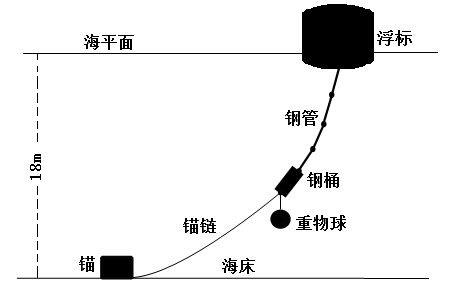
\includegraphics[width=0.8\textwidth]{img/title.jpg}
\caption{传输节点示意图(仅为结构模块示意图,未考虑尺寸比例)}\label{fig-buoy}
\end{figure}	

\begin{enumerate}[(1)]
	\item 假设海水静止,给定锚链链长、重物球质量和水深,要求在不同的海风风速条件下,求出钢桶和各节钢管的倾斜角度、锚链形状、浮标的吃水深度和游动区域。
	\item 同问题1的假设,计算给定海面风速为条件下钢桶和各节钢管的倾斜角度、锚链形状和浮标的游动区域。并要求调节重物球的质量,满足系泊系统设计的角度限制。
	\item 考虑潮汐等因素的影响,假设给定水深、海水速度和风速等参数的范围。要求给出考虑各参数约束条件下的系泊系统设计,同时分析不同情况下钢桶、钢管的倾斜角度、锚链形状、浮标的吃水深度和游动区域。
\end{enumerate}

\section{模型假设}
\begin{enumerate}
	\item 不考虑海风对于水面的影响,即不考虑波浪的影响。
	\item 将题目中浮标、钢管、钢桶视为刚体,即不考虑由于力的作用发生的形变影响。
	\item 忽略锚链的体积,即不考虑海水对锚链的摩擦力
	\item 假设稳定情况下浮标不会发生倾斜
	\item 将锚链简化为一根柔性绳
	\item 当地中立加速度为$g=9.8kg/m^3$
	\item 不考虑倾斜的海底,均视为平坦的海底进行建模
\end{enumerate}
\section{假设说明}
\begin{enumerate}
	\item 由论文\cite{floatmodel}知浮标重心比较复杂,考虑浮标发生倾斜将会使得模型复杂化,因此我们假设浮标不发生倾斜。
	\item 锚链每节长度($0.078m\sim 0.18m$)相对于总长度($22.05m$)比例较小,可以看着柔性绳。
	
\end{enumerate}
\section{符号说明}
表\ref{table-symbol}列出了本文需要的符号。
\begin{table}[H]
	\centering
	\caption{符号说明} \label{table-symbol}
	\begin{tabular*}{\textwidth}{cc||cc}
		\hline
		符号 & 符号描述 & 符号 & 符号描述 \\
		\hline
		$\rho$ & 海水密度 & $F_{fl}$ & 浮标所受浮力\\
		$v$ & 风速& $F_{p}$ & 钢管所受浮力\\
		$H$ & 浮标高度 & $F_{b}$ & 钢桶所受浮力\\
		$h$ & 浮标水上高度& $F_{s}$ & 重物球所受浮力\\
		$h_{below}$ & 吃水深度 & $F_w$ & 近海风荷载\\
		$d_{fl}$ & 浮标外径&$a$ & 悬链线参数\\
		$l_b$ & 钢桶长度& $T_{ix}$ & 节点$i(i=1,2,\dots6)$处拉力的$x$方向分量(对上)\\
		$d_b$ & 钢桶外径& $T_{iy}$ & 节点$i(i=1,2,\dots6)$处拉力的$y$方向分量(对上)\\
		$l_p$ & 钢管长度&$T_{ix}^{'}$ & 节点$i(i=1,2,\dots6)$处拉力的$x$方向分量(对下)\\
		$d_p$ & 钢管外径&$T_{iy}^{'}$ & 节点$i(i=1,2,\dots6)$处拉力的$y$方向分量(对下)\\
		$L$ & 锚链总长度& $\theta_i$ & 钢管$i$与竖直方向的夹角,即倾斜角($i=1,2,3,4$)\\
		$L_{0}$ & 锚链沉底长度&$\theta$ & 钢桶与竖直方向的夹角\\
		$L_{right}$ & 锚链未沉底长度 & $g$ & 重力加速度$(9.8m/s^2)$ \\
		$G_{fl}$ & 浮标的重力&$\beta$ & 锚链与锚连接处的切线方向与海床的夹角($0\le\beta\le16$\\
		$G_{p}$ & 钢管的重力&$B$ & 锚链底部与锚连接点\\
		$G_{b}$ & 钢桶的重力&$B^{'}$ & 锚链有一部分沉底时,沉底段与悬浮段交接点\\
		$G_{s}$ & 重物球的重力&$distance$ & 浮标与锚的水平距离\\
		$G_{c}$ & 锚链的重力& $w$ & 锚链单位长度重力\\
		\hline
	\end{tabular*}
\end{table}

\section{问题分析}
\subsection{问题一的分析}
由于题目假设,海水静止,海风分为$12m/s$和$24m/s$两种情况,我们直接求解系统在风力作用吓达到稳定时刻的状态,则该问题可以转换为简单的系统静态受力问题。由此我们可以根据受力分析对问题进行求解。\par
为方便叙述以及计算表达,我们将钢管的六个节点(包括钢管和浮标的连接点以及钢管和钢桶的连接点)由上到下依次设为节点1,节点2,\dots,节点6。以锚所在处为原点,以水平方向和竖直方向分别作为$x$轴和$y$轴在二维平面内建立正交直角坐标系,并对每一个节点受力进行正交分解。设浮标露出水面的高度为$h$,并作为唯一自变量我们可以表示出各个待求物理量。步骤如下:
\begin{enumerate}
	\item 对浮标在两个分量上进行力平衡分析。由于风力重力均已知,浮力可以用$h$唯一表示出来,就可以确定浮标所受拉力。
	\item
	由牛顿第三定律,节点受浮标的相反作用力也可以表示成$h$的函数。由于钢管没有转动,将钢管质点化进行受力分析\ref{fig:pipe},可以依次递推出每一分母个节点的受力表达式(含$h$),分别记作$T_{2x}$,$T_{2y}$,$T_{3x}$,\dots,钢桶分析类似,受力分析图见\ref{fig:bottle}。
	\item
	然后根据钢管、钢桶不转动,即力矩平衡\cite{physics}可以得到各个部分与水平部分所成的倾角$\theta_1$,\\$\theta_2,\theta_3,\dots$ 。钢桶也可作类似分析。
	\item
	接着关于锚链建立悬链线模型。锚链由于被看作是柔性线,每一点受力均沿着锚链切线方向。因此用已知的受力关系可以由h表示出悬链线方程。锚链可能出现两种状态:左侧有沉底和锚链全部悬浮在水中两种情况。为此我们建立了两个模型进行分别计算,再将锚链右侧端点的坐标表示成$h$的表达式。
	\item
	由此我们可以将系统中每一部分的y方向投影计算出来,由水深18m这个限制条件利用Matlab的fsolve指令进行计算即可求解$h$的值,于是求出题目中要求的变量。经过计算我们得出:风速为12m/s时,锚链左侧一部分沉底,风速为24m/s时,锚链全部飘起。
\end{enumerate}
\begin{figure}[H]
  \begin{minipage}[t]{0.5\linewidth}   
    \centering   
    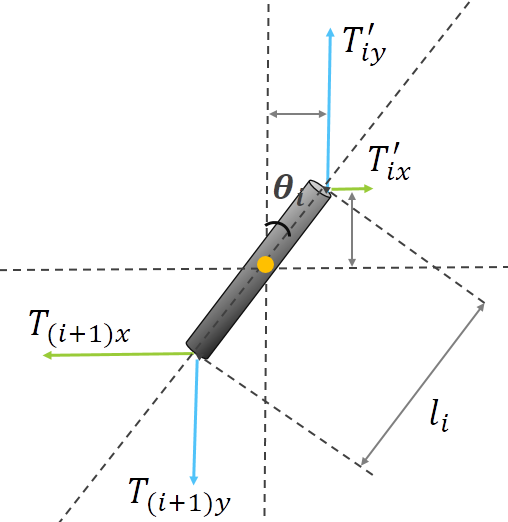
\includegraphics[width=0.8\textwidth]{img/pipe.png}   
    \caption{钢管受力分析图}   
    \label{fig:pipe}   
  \end{minipage}   
   \begin{minipage}[t]{0.5\linewidth} % 如果一行放2个图,用0.5,如果3个图,用0.33  
      \centering   
      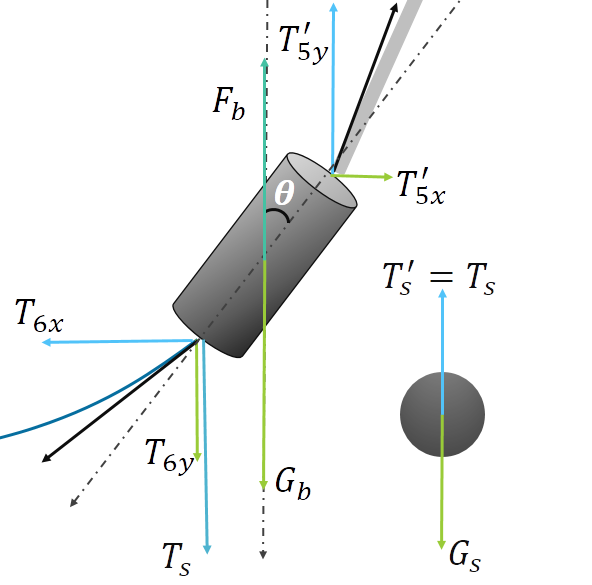
\includegraphics[width=0.8\textwidth]{img/bottle.png}   
      \caption{钢桶受力分析图}   
      \label{fig:bottle}   
    \end{minipage} 
\end{figure}


\subsection{问题二的分析}
问题二第一问即将风速代入问题一求出的模型,计算结果。\par 
对于第二问,我们从直观上来分析:风力一定的情况下,如果重物球质量较轻,从锚链到钢桶,再到钢管都可能被拉大角度,$\beta$角和$\theta$角即有可能超过限制。故需要增大重物球质量,使其达到可行解域,可知重物球质量是有下限值的。另一方面,浮标和其他物体的浮力有限,重物球的质量一定不能超过其最大浮力,故其也有上限。\par 
对这个问题,我们的解决方法是通过粗略作图确定大致上限和下限,再通过二分法搜索出其精确值。
\subsection{问题三的分析}
问题三有四个目标变量,分别是浮标的吃水深度、浮标的游动区域和钢桶的倾斜角度以及锚链底端切线水平仰角。同时又六个自变量,分别是风速、水速、水深、锚链型号、锚链长度、重物球重量。由于自变量数目较多,并且不同自变量对不同目标变量的影响大小不同,我们采用逐步优化的方式,先固定某几个自变量,分析另外几个自变量对目标变量的影响。\par
\begin{enumerate}
	\item 自变量的选取与初步分析 \par 
	首先选择最重要的两个自变量,锚链长度和重物球重量作为分析对象。考虑锚链型号为II、最大风速、最大水速和水深为18米的情况下,不同锚链长度和重物球重量对四个目标量的影响,作出四个三维图像,考虑钢桶倾角$\theta$和锚链底端切线水平仰角$\beta$的限制,通过观察图像,分析出可行解的范围。\par 
	\item 确定可行解域中最优解的分布\par 
	在可行解的范围中,易分析出取得最优解一定是在可行解域边界上。由于题目中对$\beta$只有限制而不做优化要求,故最优解一定是在使$\beta =16$的值上,称最优解域。\par 
	\item 确定多目标的目标函数并求出最优解\par 
	可以从图\ref{fig:2_18_theta}和图\ref{fig:2_18_h}看出,两者在水平方向的变化趋势是向同的,而$h_{below}$与$h$的变化趋势相反,故$\theta$和$h$的目标也相反。因此我们设定了一个目标函数将这两者分配权重结合起来考虑。再通过计算最优解域上的目标函数值找到最优解。
\end{enumerate}\par 
以上为对自变量锚链长度和重物球重量最优解的求解方法,之后对于不同锚链型号和不同水深的情况也将用此方法求解出最优解的两个值,共15组解,每组解分别具有一个评价函数值和浮标的游动区域值。\par
\begin{enumerate}
	\item 确定水深对最优解的影响\par 
	对于水深会变化的水域,可行解域有所不同,应该考虑对任何情况下都在可行解域中的解。\par 
	\item 确定锚链型号\par 
	
\end{enumerate}



\section{问题的解答}
\subsection{问题1的解答}
在海水静止的条件下,以锚所在处为坐标原点,以水平方向为$x$轴,以竖直方向为$y$轴,在二维平面内建立正交直角坐标系,将浮标与锚链之间的六个节点由上到下依次设为节点1,节点2,\dots,节点6,假设浮标露出水面的高度为$h$。

\subsubsection{模型的准备:悬链线模型}\label{model}
对于单锚链的研究,计算方法参考\cite{seaStructure}\par 
\begin{figure}[h]
  \begin{minipage}[t]{0.5\linewidth}   
    \centering   
    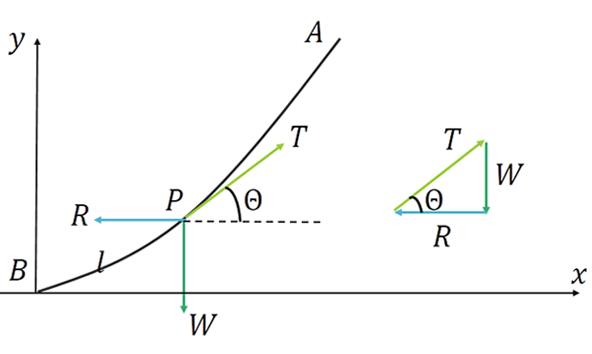
\includegraphics[width=0.8\textwidth]{img/rope_strength.png}   
    \caption{悬链线基本模型}   
    \label{fig:rope_strength}   
  \end{minipage}   
   \begin{minipage}[t]{0.5\linewidth} % 如果一行放2个图,用0.5,如果3个图,用0.33  
      \centering   
      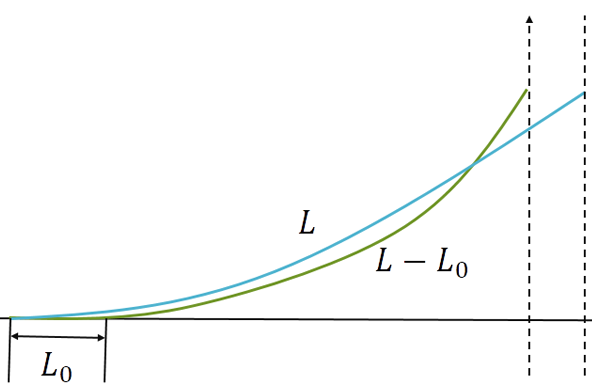
\includegraphics[width=0.8\textwidth]{img/rope_dif.png}   
      \caption{悬链线沉底情况}   
      \label{fig:rope_lying}   
    \end{minipage} 
\end{figure}

图\ref{fig:rope_strength}中AB是一条悬链线,A与水中漂浮结构连接,B点与锚相连并且与海底相切,单位长链重量为$w$,对于线中P点,我们可以看作一个新的漂浮结构。把PB看为一个整体,长度为$l$,那么,$P$点所受张力$T$、$PB$链重力$W(W=wl)$和水平系泊力$R$处于平衡状态。因为$\tan{\theta}=\dfrac{dx}{dy}$ ,考虑力三角平衡条件,可得

\begin{displaymath}
	\dfrac{dx}{dy}=\tan{\theta}=\dfrac{W}{R}=\dfrac{wl}{R}\label{12-55}
\end{displaymath}
又
\begin{displaymath}
	dl=\sqrt{(dx)^2+(dy)^2}
\end{displaymath}
所以
\begin{displaymath}
	\dfrac{dl}{dx}=\sqrt{1+(\frac{dy}{dx})^2}
\end{displaymath}
对式\ref{12-55}两边取微分,便可得到悬链线微分方程如下:
\begin{displaymath}
	\dfrac{d^2y}{d^2x}=\dfrac{w}{R}\dfrac{dl}{dx}=\dfrac{w}{R}\sqrt{1+(\dfrac{dy}{dx})^2}
\end{displaymath}
令$\dfrac{dy}{dx}=f,\dfrac{d^2y}{d^2x}=\dfrac{f}{x}$,则上式变为
\begin{displaymath}
	\dfrac{df}{dx}=\dfrac{w}{R}\sqrt{1+f^2}
\end{displaymath}
积分上式,并根据初始条件,$x=0,\dfrac{dy}{dx}=0$,可知上式的积分常数为零,于是得
\begin{displaymath}
	\dfrac{dy}{dx}=\sinh(\dfrac{w}{R}x)
\end{displaymath}
再次积分上式,得
\begin{displaymath}
	y=\dfrac{R}{w}\cosh(\dfrac{w}{R}x)+C_1
\end{displaymath}
由于$x=0$时,$y=0$,所以$C_1=-\dfrac{R}{w}$,于是得悬链线方程
\begin{displaymath}
	y=\dfrac{R}{w}\cosh(\dfrac{w}{R}x)-\dfrac{R}{w}
\end{displaymath}
引入参数$a=\dfrac{R}{w}$,称为悬链线参数,则有
\begin{equation}
	y=\dfrac{R}{w}\cosh(\dfrac{w}{R}x)-a
	\label{eq:chain_basic}
\end{equation}
于是我们得到最基础的悬链线模型,悬链一头与地面相切的悬链线方程。\par 
还有另一种表示方法:
\begin{equation}
l=\dfrac{R}{w}\sinh(\dfrac{w}{R}x)
\label{eq:chain_length}
\end{equation}
可用于计算悬链线长度。
\subsubsection{模型计算}
浮标受力如图\ref{fig:float}
\begin{figure}[H]
	\centering
	\includegraphics*[width=0.3\textwidth]{img/float.png}
	\caption{浮标受力分析图}
	\label{fig:float}
\end{figure}
$F_w=0.625\times Sv^2$,浮标所受浮力为$F_{fl}=(2-h)\pi \frac{d_{fl}^2}{4} \rho  g(N)$,浮标重力$G_{fl}=1000g$。首先对浮标在两个方向上进行受力分析,有等式
\begin{displaymath}
\left\{
\begin{aligned}
	F_{fl} &=T_{1y}+G_{fl}\\
	T_{1x} &=F_w\\
\end{aligned}
\right.
\end{displaymath}
由此可得
\begin{displaymath}
\left\{
\begin{aligned}
	T_{1x} &=720h\\
	T_{1y} &=(2-h)\pi \frac{d_{fl}^2}{4} \rho g-1000g
\end{aligned}
\right.
\end{displaymath}
其中$\rho$为海水的密度,$g$为重力加速度。对于接下来四根钢管的受力分析可以采用递推的模型,对于第$i(i=1,2,3,4)$根钢管的受力平衡方程为,其中$T_i$与$T_i^{’}$大小相等,方向相反,为一对相互作用力。
\begin{displaymath}
\left\{
\begin{aligned}
	T_{ix}^{'}&=T_{(i+1)x}\\
	T_{iy}^{'}&=G_p+T_{(i+1)y}
\end{aligned}
\right.
\end{displaymath}
然后对于钢桶的力平衡方程为
\begin{displaymath}
\left\{
\begin{aligned}
	&T_{5x}^{'}=T_{6x}\\
	&T_{5y}^{'}+F_b+F_s=G_s+G_b+T_{6y}
\end{aligned}
\right.
\end{displaymath}
式中
对于锚链的分析需要先建立一个悬链线模型与\ref{eq:chain_basic}相类似,需要注意的是,该模型适用条件是锚链底端和海底相切。因此应将模型稍作修改。
\begin{itemize}
\item \textbf{情况一:悬链无沉底部分}\par
假设该点处悬链线不沉底,如图\ref{fig:rope_strength}所示,悬链线的切线与水平方向成$\beta(\beta>0)$角,悬链线总长为$L_c$。取悬线上某一点$P$,$PB$长度为$l$,设$P$点处切线方向与水平方向夹角为$\alpha$,此时$P$点受力的垂直分量与悬链线底端受力垂直分量和悬链线重力之和相等。从而有
\begin{displaymath}
	\dfrac{dy}{dx}=\tan{\alpha}=\dfrac{wl+R\tan{\beta}}{R}
\end{displaymath}
令$k=\tan{\beta}$,得到
\begin{displaymath}
	\dfrac{dy}{dx}=\dfrac{Rk+wl}{R}=\dfrac{wl}{R}+k
\end{displaymath}
对上式两边求导
\begin{displaymath}
	\dfrac{d^2y}{dx^2}=\dfrac{w}{R}\dfrac{dl}{dx}=\dfrac{w}{R}\sqrt{1+(\dfrac{dy}{dx})^2}
\end{displaymath}
再令$f=\dfrac{dy}{dx}$,得到
\begin{displaymath}
	\dfrac{df}{\sqrt{1+f^2}}=\dfrac{w}{R}dx
\end{displaymath}
对上式两边积分即有
\newcommand{\arcsinh}{\mathrm{arcsinh}\,}
\begin{displaymath}
	\arcsinh(f)+C=\dfrac{w}{R}x
\end{displaymath}
其中$C$为常数,由初始条件$x=0$时$f=k$得出$C=-\arcsinh(k)$,整理后,令$a=\dfrac{R}{w}$有
\begin{displaymath}
	\dfrac{y}{x}=f=\sinh(\dfrac{x}{a}+\arcsinh(k))
\end{displaymath}
通过积分得到适用模型
\begin{align}
	y=ak\sinh(\dfrac{x}{a})+a\cosh(\dfrac{x}{a})\sqrt{k^2+1}-a\sqrt{k^2+1}\label{model:full}
\end{align}
\item \textbf{情况二:悬链部分沉底}\\
当锚链部分沉底时,如图\ref{fig:rope_lying}所示,记沉底部分长度为$L_0$,则$(L-L_0)*w=T_{6y}^{'}$,其中$w$为单位长度锚链重力。悬链线方程套用基本模型\ref{eq:chain_basic}即可。
\item \textbf{锚链是否沉底的判别方法}
可先假设其为沉底的情况。如果锚链有一部分沉底,则先使用基本模型\ref{eq:chain_basic},以第六个节点的横坐标为自变量并解出它,将其代入方程\ref{eq:chain_length}得到锚链未沉底的长度$L_{right}$,对其进行判断,如果其符合条件$L \ge L_{right},L_{right} \ge 0$即认为计算有效,否则使用模型\ref{model:full} 
\end{itemize}\par 
先考虑悬链不发生沉底的情况。
对于节点6处,受力方向沿悬链线切线方向,由此得$\dfrac{dy}{dx}=\dfrac{T_{6y}^{'}}{T_{6x}^{'}}$代入式\ref{model:full},即可得到$x,y$关于$h$的表达式。\\
接下来对四根钢管由图\ref{fig:pipe_m}分析,列出力矩平衡的方程
\begin{displaymath}
	T_{ix}^{'}\cos{\theta_i}+0.5G_p\sin{\theta_i}=T_{iy}^{'}\sin{\theta_i}+0.5F_p\sin{\theta_i}(i=1,2,3,4)
\end{displaymath}
\begin{figure}[H]
	\centering
	\includegraphics*[width=0.4\textwidth]{img/pipe_m.png}
	\caption{钢管力矩平衡示意图}
	\label{fig:pipe_m}
\end{figure}
再根据钢桶力矩平衡得到
\begin{displaymath}
	T_{5x}^{'}\cos{\theta}+0.5G_b\sin{\theta}=T_{5y}^{'}\sin{\theta}+0.5F_b\sin{\theta}
\end{displaymath}
由此得到四根钢管和钢桶的倾斜角余弦表达式
\begin{equation}
\left\{
\begin{aligned}
&\cos{\theta_1}=\sqrt{\frac{1}{\frac{25\, {d_{f}l}^2\, h^2\, v^4}{16\, {\left( - \frac{g\, \mathrm{\rho}\, \pi\, \left(H - h\right)\, {d_{f}l}^2}{2} + 2\, G_{f}l + G_{p} - \frac{\pi\, g\, \mathrm{\rho}}{1600}\right)}^2} + 1}}\\
&\cos{\theta_2}=\sqrt{\frac{1}{\frac{25\, {d_{f}l}^2\, h^2\, v^4}{16\, {\left( - \frac{g\, \mathrm{\rho}\, \pi\, \left(H - h\right)\, {d_{f}l}^2}{2} + 2\, G_{f}l + 3\, G_{p} - \frac{3\, \pi\, g\, \mathrm{\rho}}{1600}\right)}^2} + 1}} \\
&\cos{\theta_3}=\sqrt{\frac{1}{\frac{25\, {d_{f}l}^2\, h^2\, v^4}{16\, {\left( - \frac{g\, \mathrm{\rho}\, \pi\, \left(H - h\right)\, {d_{f}l}^2}{2} + 2\, G_{f}l + 5\, G_{p} - \frac{\pi\, g\, \mathrm{\rho}}{320}\right)}^2} + 1}} \\
&\cos{\theta_4}=\sqrt{\frac{1}{\frac{25\, {d_{f}l}^2\, h^2\, v^4}{16\, {\left( - \frac{g\, \mathrm{\rho}\, \pi\, \left(H - h\right)\, {d_{f}l}^2}{2} + 2\, G_{f}l + 7\, G_{p} - \frac{7\, \pi\, g\, \mathrm{\rho}}{1600}\right)}^2} + 1}}\\
&\cos{\theta}=\sqrt{\frac{1}{\frac{25\, {d_{f}l}^2\, h^2\, v^4}{16\, {\left( - \frac{g\, \mathrm{\rho}\, \pi\, \left(H - h\right)\, {d_{f}l}^2}{2} + G_{b} + 2\, G_{f}l + 8\, G_{p} - \frac{11\, \pi\, g\, \mathrm{\rho}}{400}\right)}^2} + 1}}
\end{aligned}
\right.
\end{equation}
最后根据方程
\begin{equation}
H-h+l_p(\cos{\theta_1}+\cos{\theta_2}+\cos{\theta_3}+\cos{\theta_4})+l_b\cos{\theta}+y=18
\label{eq:restrain}
\end{equation}
解方程\ref{eq:restrain}得到$\beta<0$,与假设不符。由此我们认为锚链有一部分沉底。设沉底长度为$L_0$,满足$L-L_0=\frac{T_{6y}^{'}}{w}$,我们以沉底段与悬浮段交接点$B^{'}$为坐标原点,套用基本公式\ref{eq:chain_basic},利用约束条件\ref{eq:restrain}进行求解。结果如表\ref{table:result_1}和表\ref{table:pipe_angle}。锚链形状如图\ref{fig:chain_shape_12ms}以及图\ref{fig:chain_shape_24ms}

\begin{table}[!htp]
\centering
\caption{问题一部分计算结果}\label{table:result_1}
\centering
	\begin{tabular*}{\textwidth}{cccccc}
	
		\hline
		风速$(m/s)$ & 钢桶倾斜角$(^\circ)$ & 吃水深度$(m)$ & 游动半径$(m)$ & 沉底长度$(m)$ & 锚链参数$a$\\
		\hline
		12 & 1.0083 & 0.7348 & 14.3051 & 6.8219 & 3.3198\\
		24 & 3.8498 & 0.7489 & 17.4255 & 0.3158 & 13.1308\\
		\hline
	\end{tabular*}
\end{table}
\begin{table}[H]
\centering
\caption{问题一钢管倾斜角计算结果}
\label{table:pipe_angle}
	\begin{tabular*}{0.85\textwidth}{ccccc}
		\hline
		风速$(m/s)$ & 钢桶倾斜角1 & 钢桶倾斜角2 & 钢桶倾斜角3 & 钢桶倾斜角4\\
		\hline
		12 & 0.9774 & 0.9832 & 0.9890 & 0.9949\\
		24 & 3.7360 & 3.7572 & 3.7787 & 3.8005\\
		\hline
	\end{tabular*}
\end{table}
\begin{figure}[H]
  \begin{minipage}[t]{0.5\linewidth}   
    \centering   
    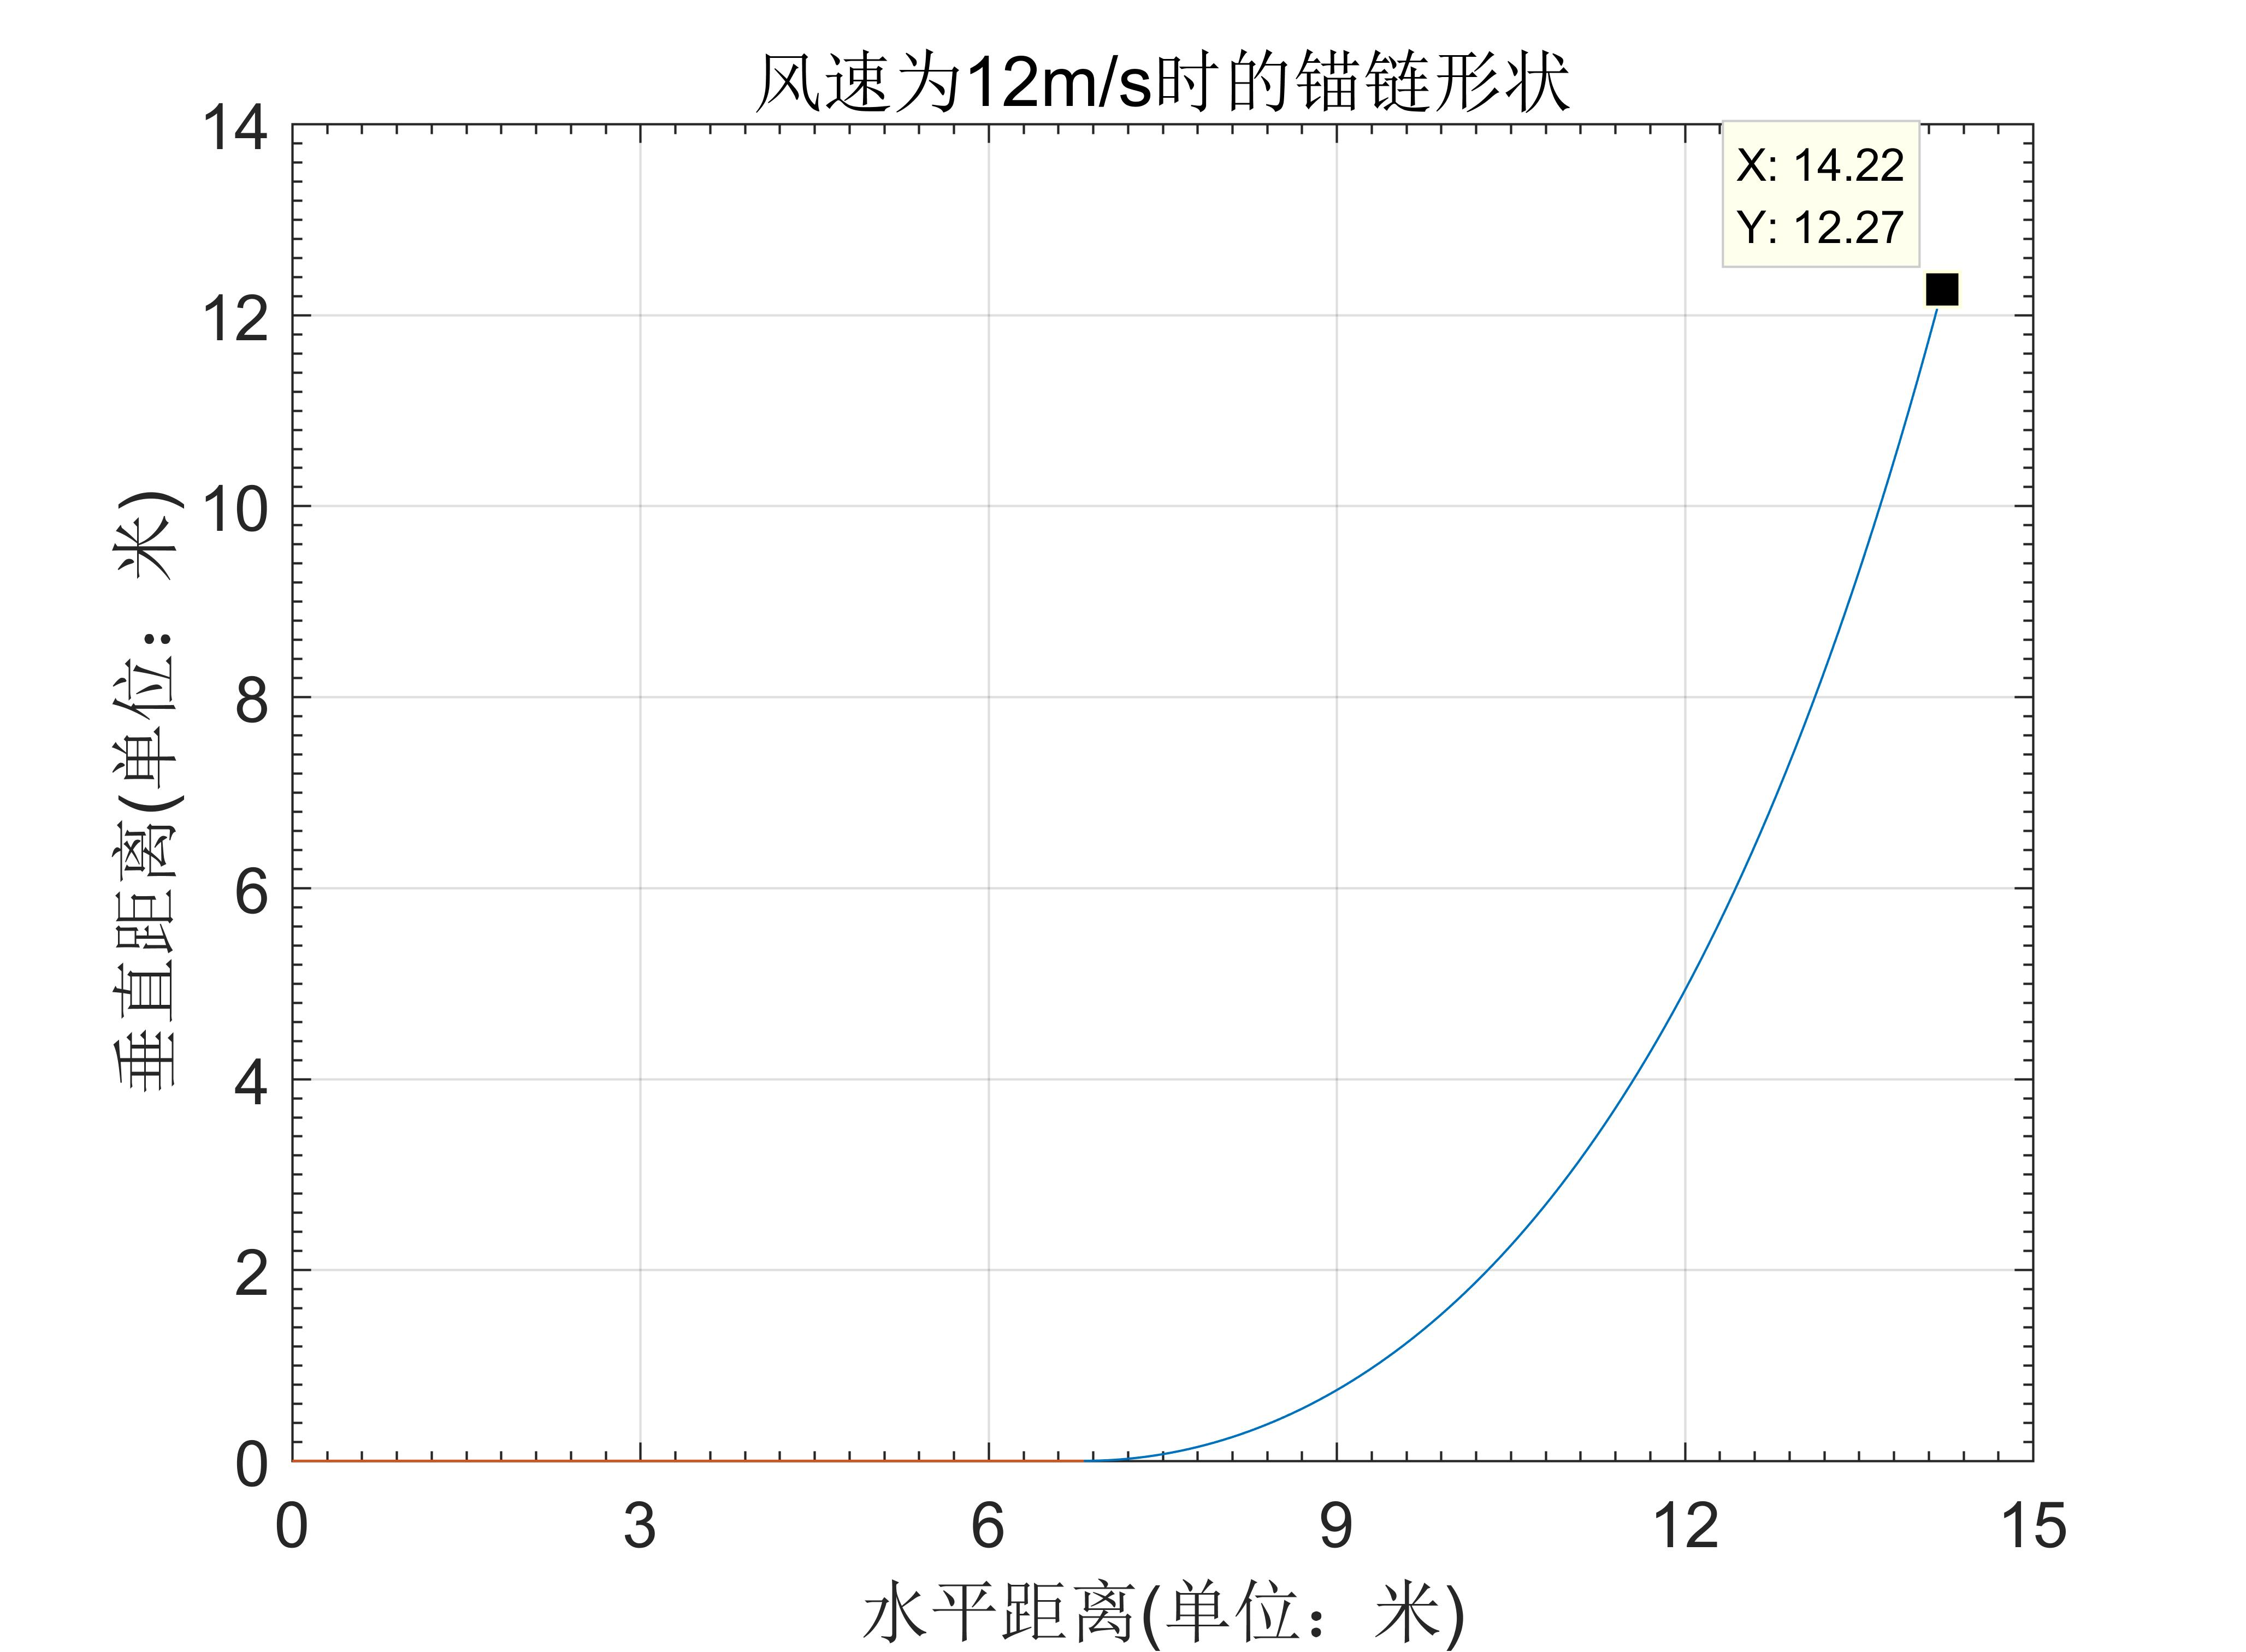
\includegraphics[width=\textwidth]{img/12mschainfigure.jpg}   
    \caption{风速为$12m/s$时锚链形状}   
    \label{fig:chain_shape_12ms}   
  \end{minipage}
   \begin{minipage}[t]{0.5\linewidth} % 如果一行放2个图,用0.5,如果3个图,用0.33  
      \centering   
      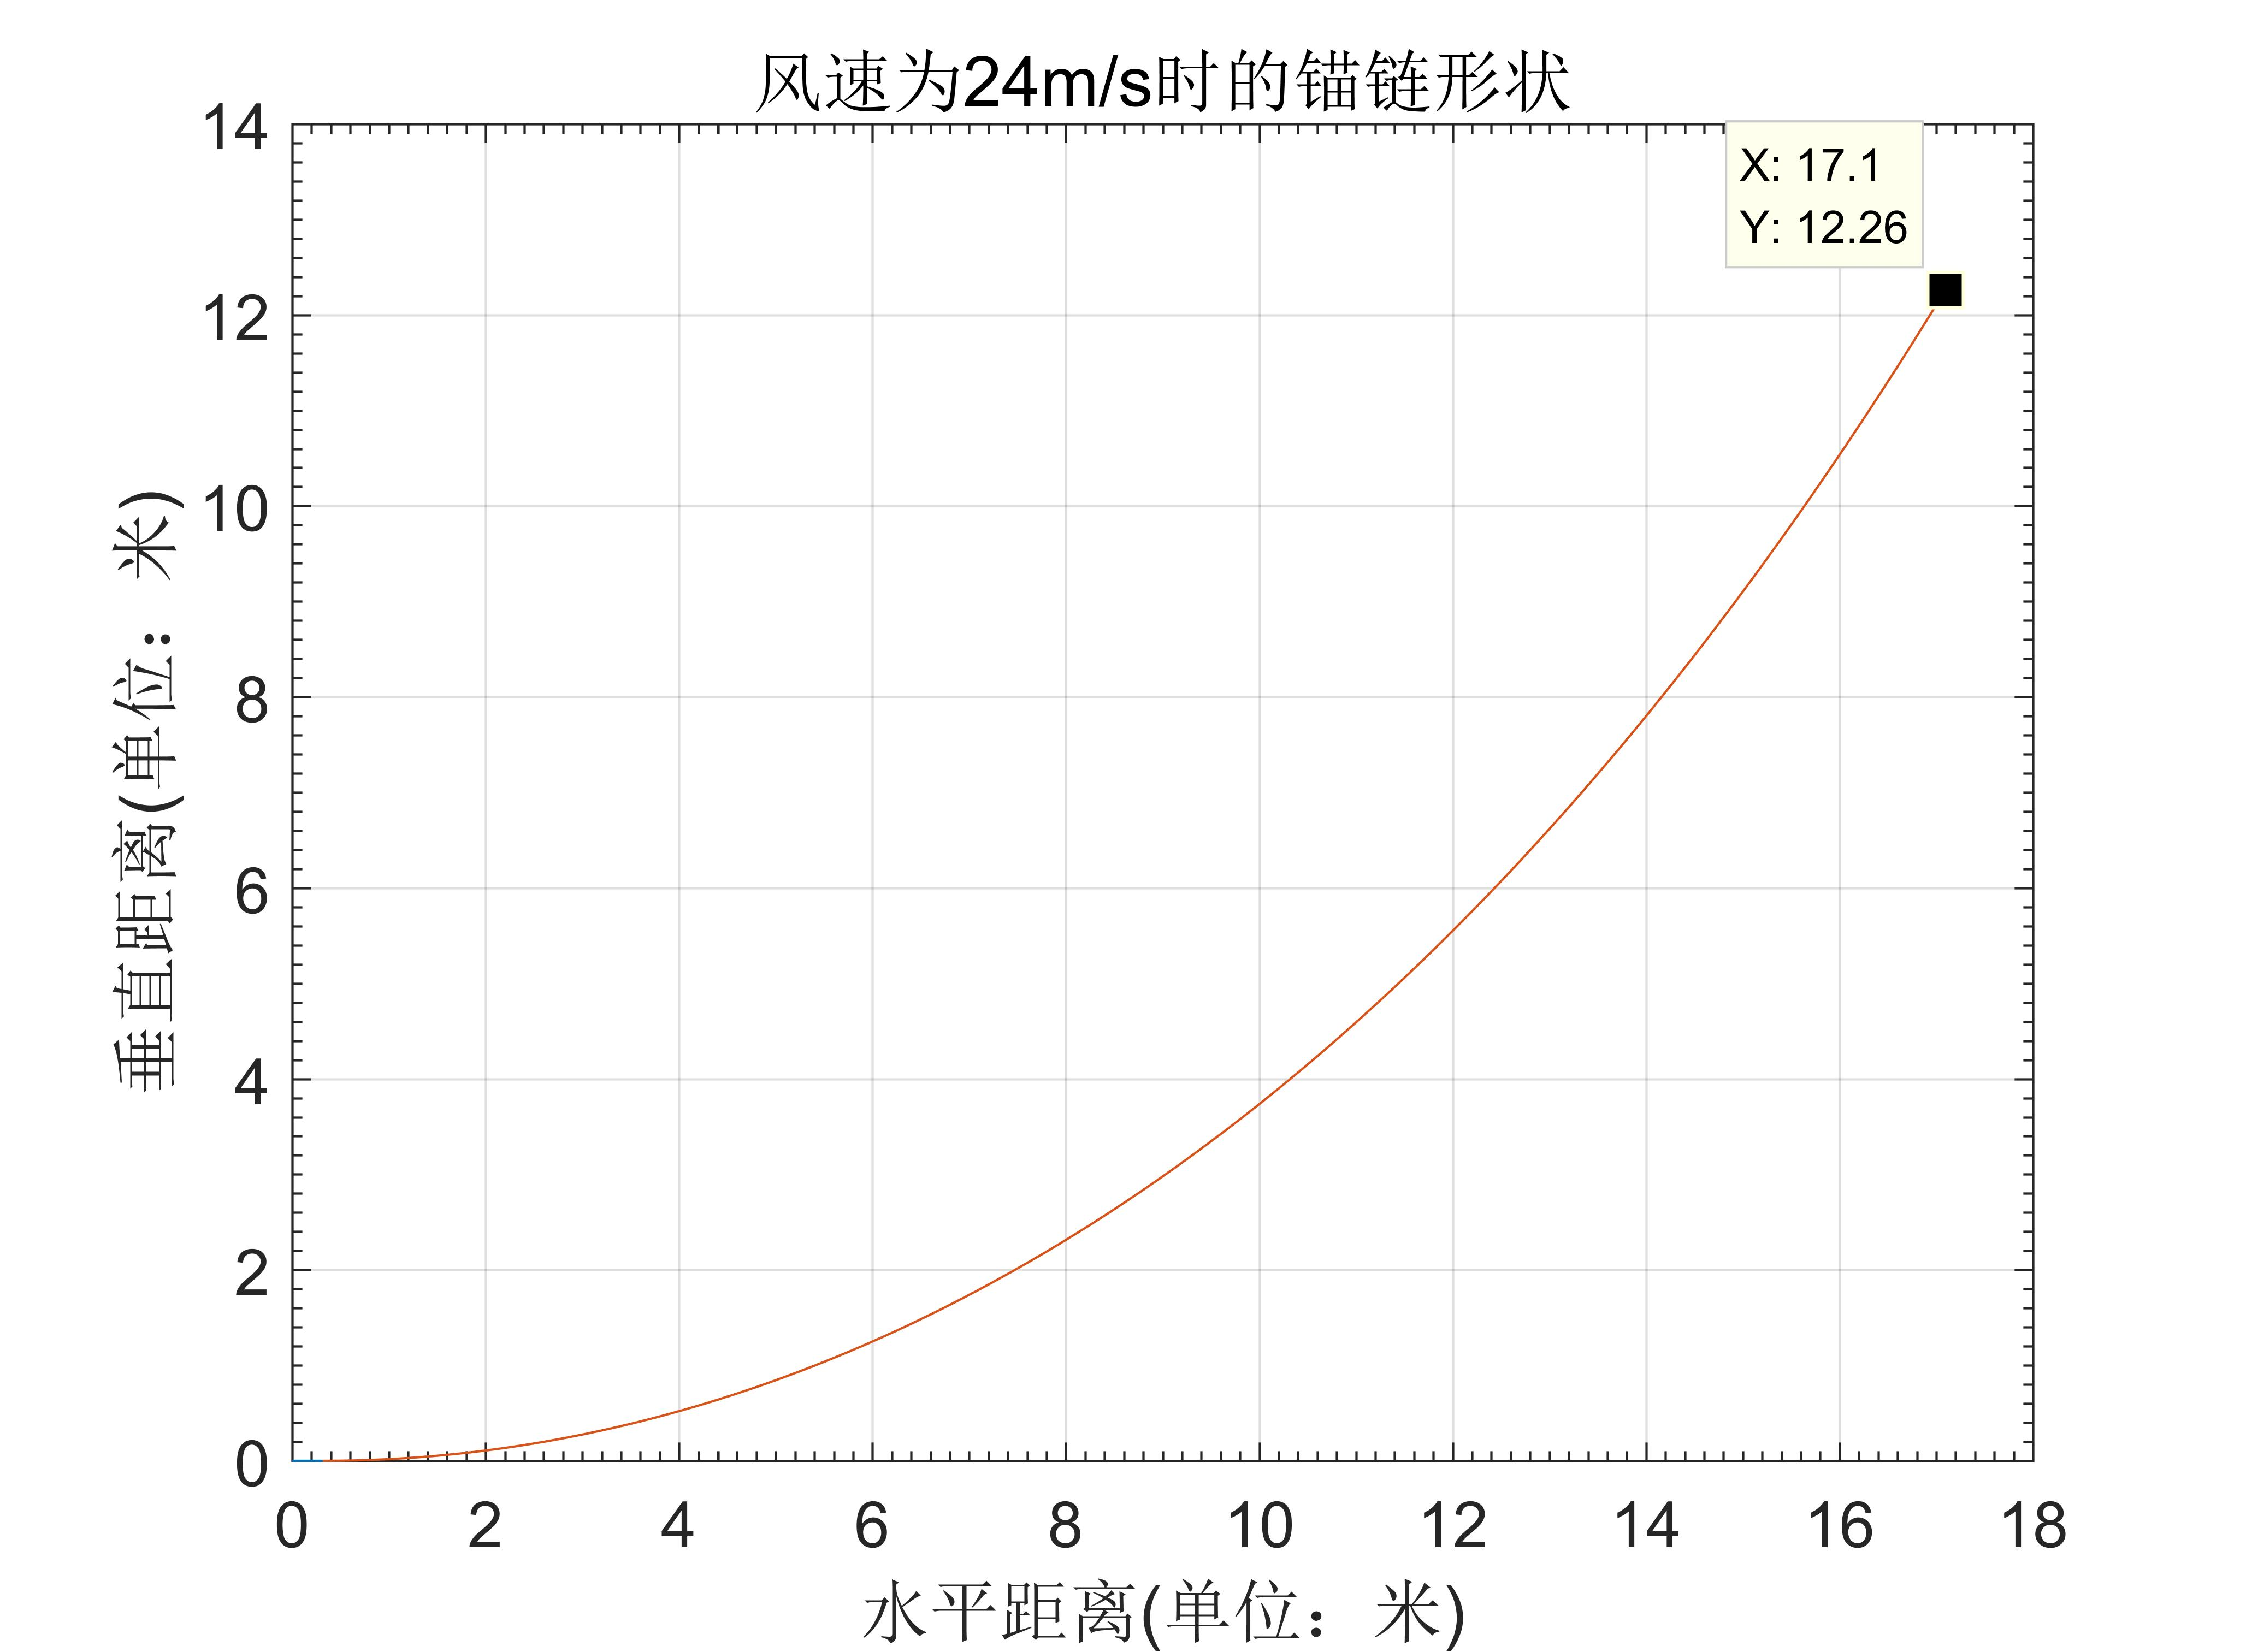
\includegraphics[width=\textwidth]{img/24mschainfigure.jpg}   
      \caption{风速为$24m/s$时锚链形状}   
      \label{fig:chain_shape_24ms}   
    \end{minipage} 
\end{figure}

\subsection{问题2的解答}
在问题一的假设下,将海面风速为36m/s时的各项计算结果如表\ref{table:result_2}和表\ref{table:pipe_angle_2},锚链形状如图\ref{fig:chain_shape_36}。
\begin{table}[!htp]
	\centering
	\caption{问题二部分计算结果}\label{table:result_2}
	\centering
	\begin{tabular*}{\textwidth}{ccccc}
		
		\hline
		风速$(m/s)$ & 钢桶倾斜角$(^\circ)$ & 吃水深度$(m)$ & 游动半径$(m)$ & 锚链参数$a$\\
		\hline
		36 & 8.0708 & 0.7700 & 18.7156  & 29.0460\\
		\hline
	\end{tabular*}
\end{table}
\begin{figure}[H]
	\centering
	\includegraphics*[width=0.5\textwidth]{img/36mschainfigure.jpg}
	\caption{风速为36$m/s$时的锚链形状}
	\label{fig:chain_shape_36}
\end{figure}
\begin{table}[H]
	\centering
	\caption{问题二钢管倾斜角计算结果}
	\label{table:pipe_angle_2}
	\begin{tabular*}{0.85\textwidth}{ccccc}
		\hline
		风速$(m/s)$ & 钢桶倾斜角1 & 钢桶倾斜角2 & 钢桶倾斜角3 & 钢桶倾斜角4\\
		\hline
		36 & 7.8454 & 7.8876 & 7.9302 & 7.9733\\
		\hline
	\end{tabular*}
\end{table}

由之前问题2的分析,我们的目标在于寻找重球重力的最小值,使得重球重力大于这个最小值时满足$\theta$和$\beta$的限制条件。\par
求$G_s$
\begin{displaymath}
	s.t.\left\{
	\begin{aligned}
	\theta\le 5^\circ\\
	\beta \le 16^\circ\\
	\end{aligned}
	\right.
\end{displaymath}
通过定长搜索得到$\theta$和$\beta$随$G_s$的变化趋势如图\ref{fig:theta_G_s}和图\ref{fig:beta_G_s}:
\begin{figure}[H]
  \begin{minipage}[t]{0.5\linewidth}   
    \centering   
    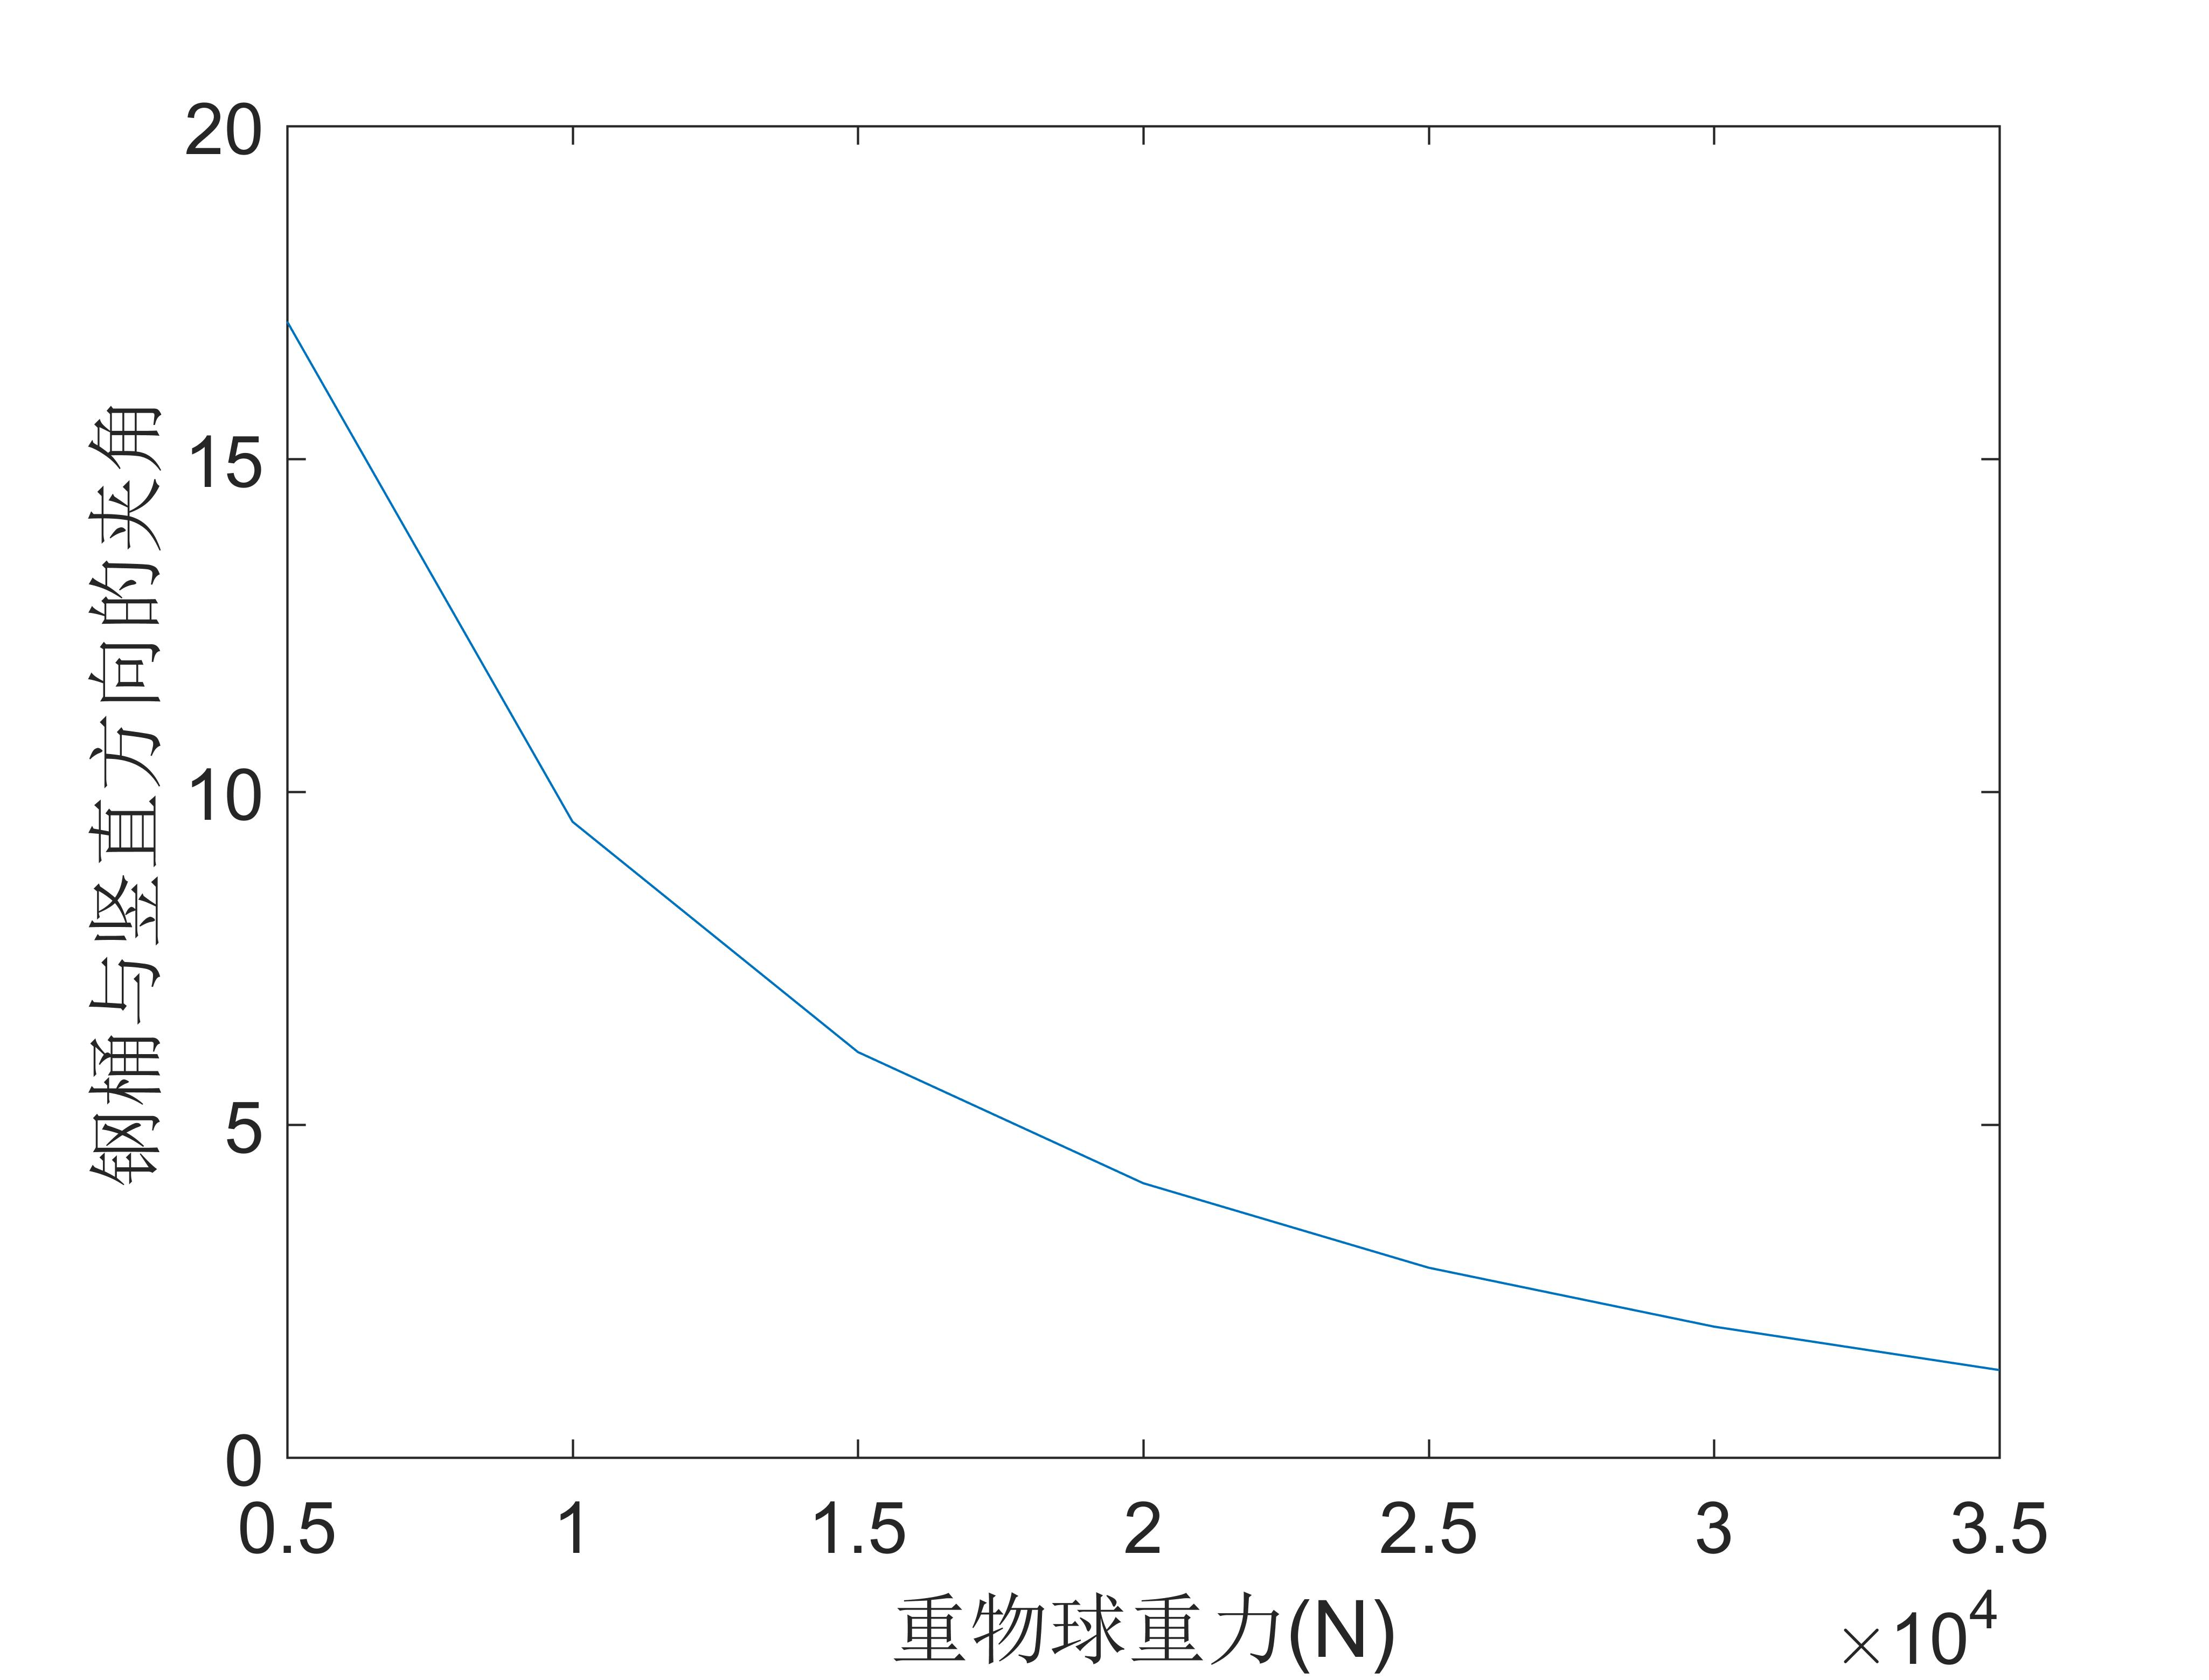
\includegraphics[width=\textwidth]{img/theta_G_s.jpg}   
    \caption{$\theta$随$G_s$变化曲线}   
    \label{fig:theta_G_s}   
  \end{minipage}
   \begin{minipage}[t]{0.5\linewidth} % 如果一行放2个图,用0.5,如果3个图,用0.33  
      \centering   
      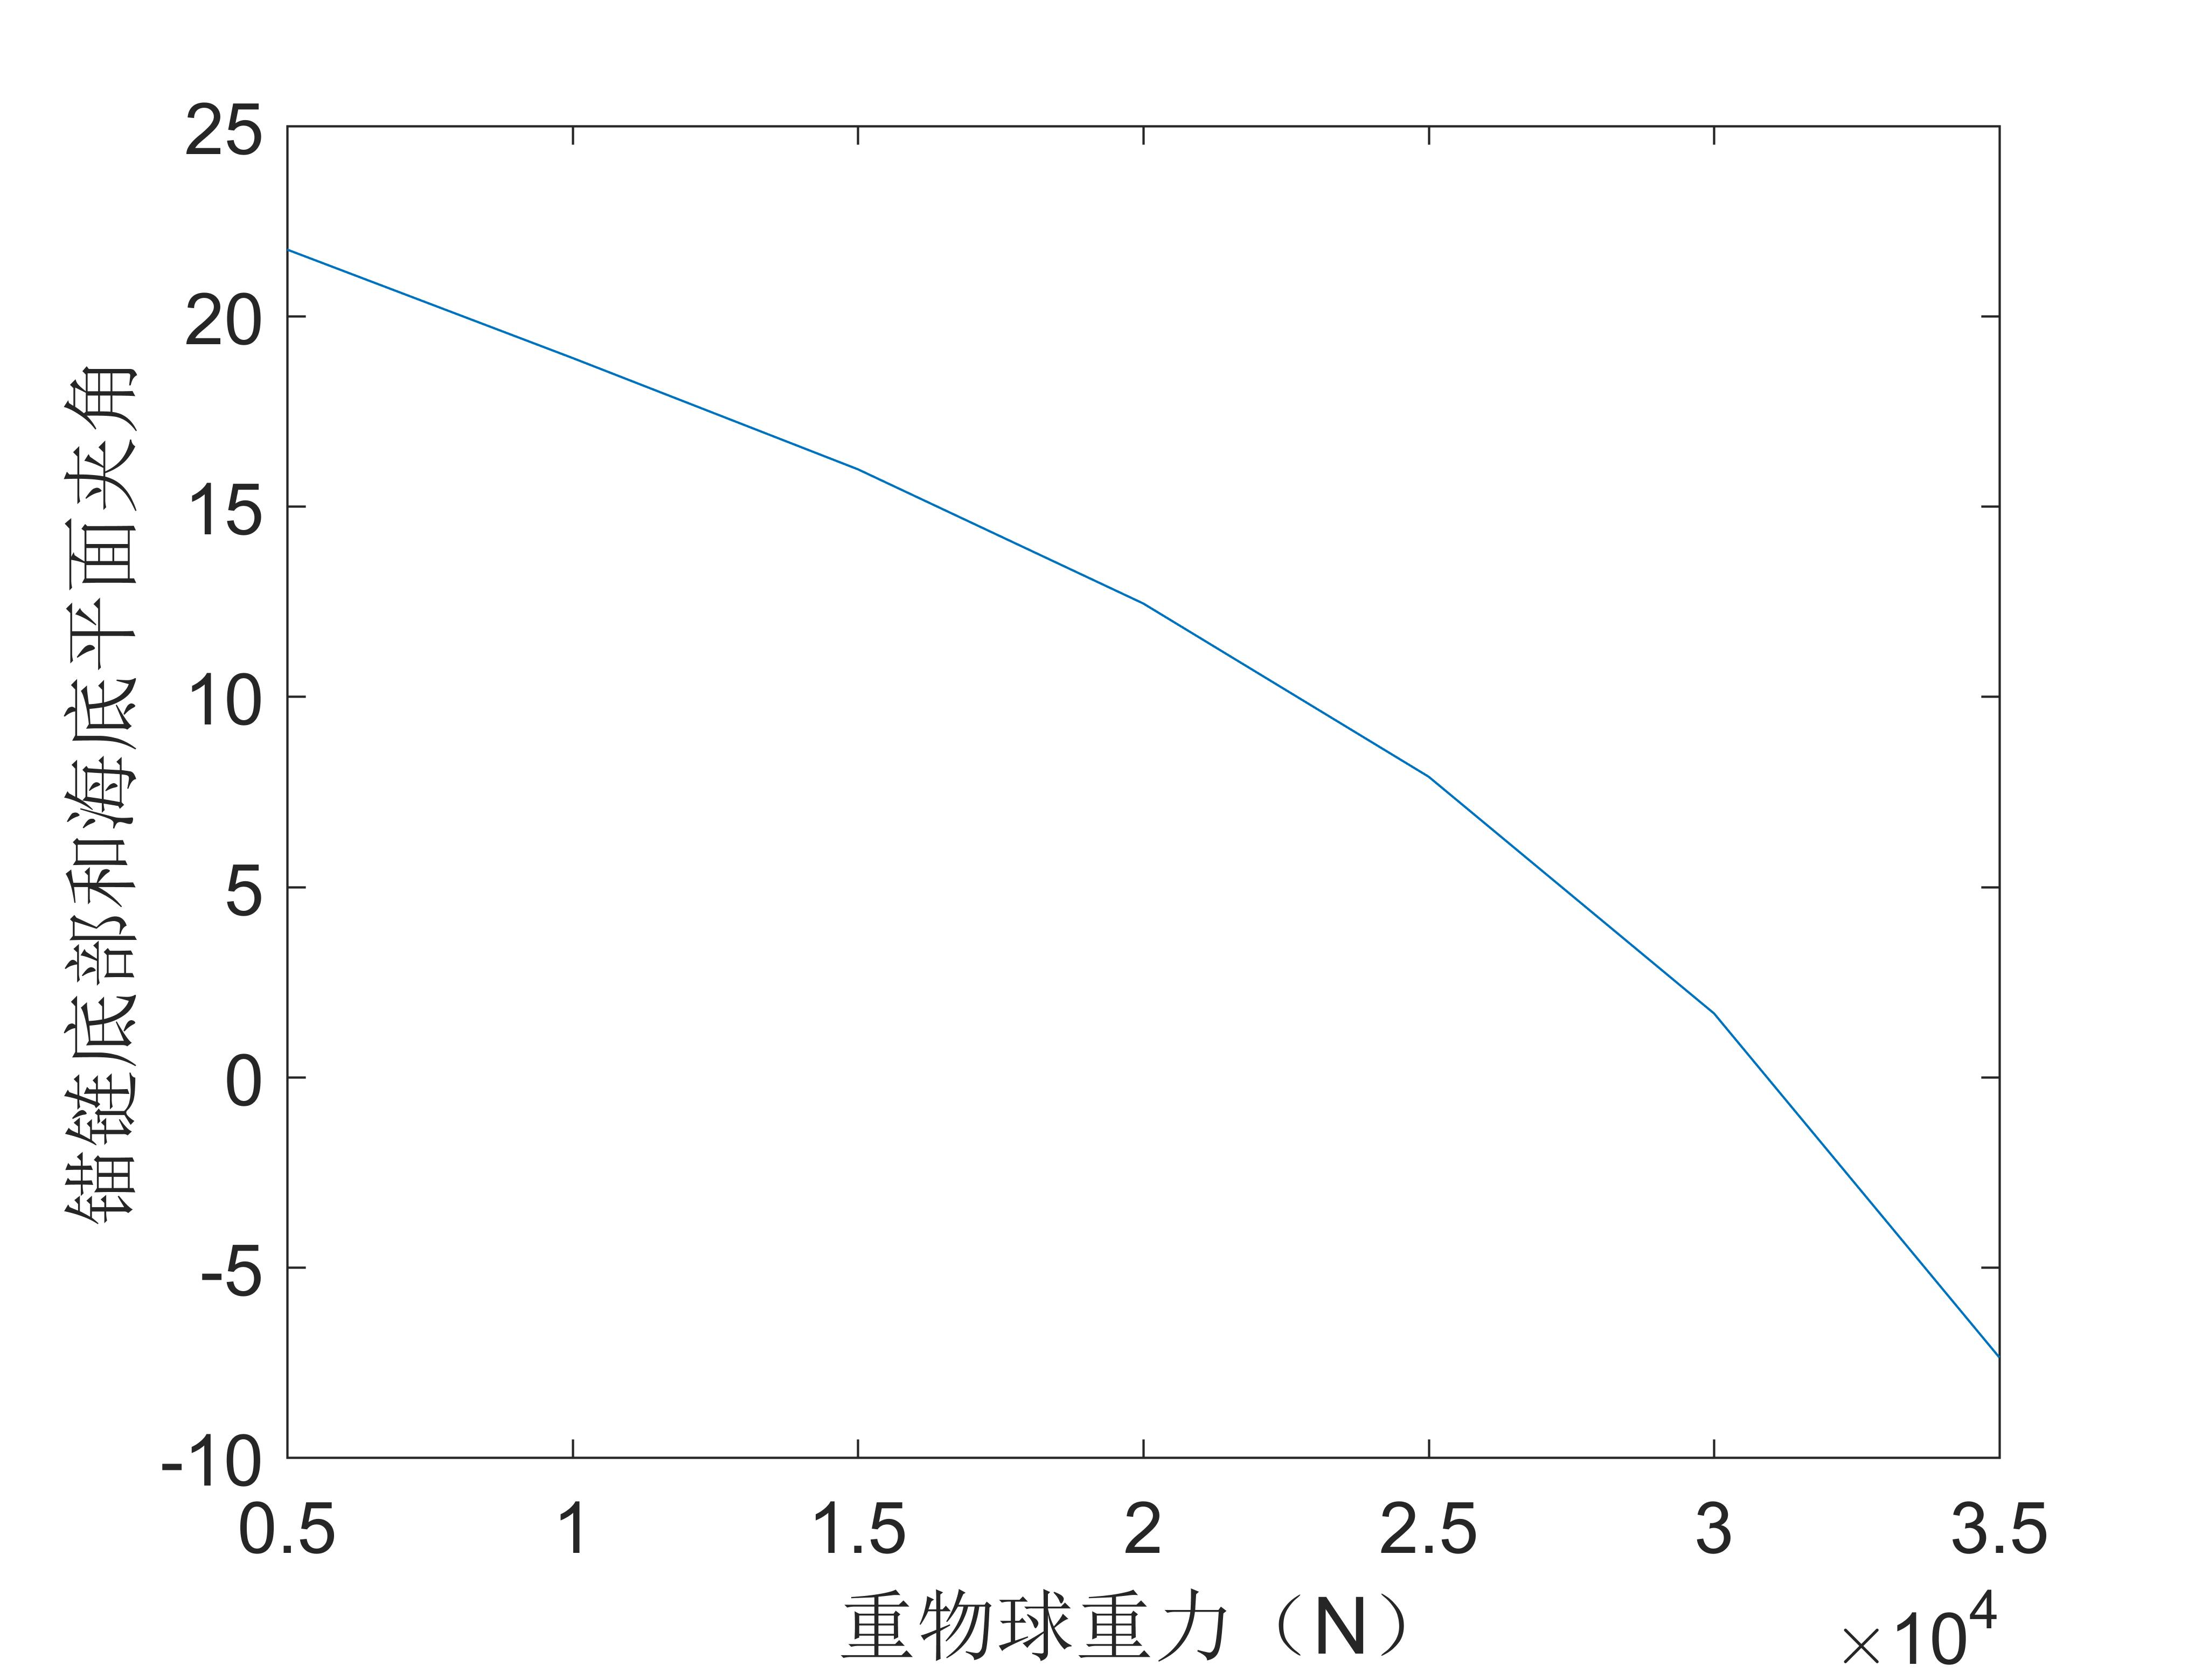
\includegraphics[width=\textwidth]{img/beta_G_s.jpg}   
      \caption{$\beta$随$G_s$变化曲线}   
      \label{fig:beta_G_s}   
    \end{minipage} 
\end{figure}
可以看到两者均为单调函数,故只有一个下限和上限,并可用二分法加快求解,算法如算法\ref{bs}:\par
\renewcommand{\algorithmicrequire}{\textbf{Input:}} 
\renewcommand{\algorithmicensure}{\textbf{Output:}}
\begin{algorithm} [H] 
	\caption{Binary search} %算法的题目 
	\label{bs} %算法的标签 
	\begin{algorithmic}[1] %此处的[1]控制一下算法中的每句前面都有标号 
		\REQUIRE {Upperbound left,lowerbound right and error restrictions $0.01$}
		\ENSURE{The weight of the ball}
		\WHILE{$|right-left|\geq0.01 \;\mathbf{and}\; angle(x_0)\neq5$}
		\IF {$angle(x_0)>5$}
		\STATE $left\leftarrow x_0$
		\ELSE
		\STATE $right\leftarrow x_0$
		\ENDIF
		\STATE $X_0\leftarrow(left+right)/2$
		\ENDWHILE
	\end{algorithmic} 
\end{algorithm}
根据图\ref{fig:theta_G_s}和图\ref{fig:beta_G_s}可对下限与上限进行二分法搜索,搜索结果为重物球质量的范围[1746.58,3172.29](单位:$kg$)。


\subsection{问题三的解答}
题目描述中,海水速度最大为$1.5m/s$,风速最大为$36m/s$。为简化模型,我们取海水速度以及风力速度均为最大值。我们将风速海速称为\textbf{环境恶劣程度}。将浮标、四节钢管看成一个整体,从直观上来看当环境越恶劣,即风速和水速越大时,这个整体受到钢桶的水平力$T_{5x}$越大,而$T_{5x}$对钢桶的力矩为顺时针转动,使得$\theta$越大,从问题一二的结果也可以验证这个猜想。故如果系泊系统在最恶劣环境下能够满足工作要求,那么系统肯定能够在平稳的环境中正常运行。\par
为了模型的建立,我们做了如下简化:
\begin{enumerate}
	\item 通过计算,水流对钢桶的力最大为$252N$,对钢管的力最大为$42N$,相对于拉力大小可以忽略不计。
	\item
	我们将水深16$m\sim 20m$的连续范围其离散化为三组$16m,18m,20m$分别进行计算。
\end{enumerate}\par 
首先我们尝试用锚链型号\uppercase\expandafter{\romannumeral2}和水深$18m$进行模型计算。由于限定了水深风速,对向量\\$(L,G_s)$($L$表示锚链长度,$G_s$表示重球质量)可以唯一确定一个系泊系统状态。我们在一定合理范围内遍历$(L,G_s)$,对钢桶倾斜角$\theta$、锚链底端切线与水平面夹角$\beta$、浮标露出水面高度$h$、浮标游动范围半径$distance$求值并作三维图像,如图\ref{fig:2_18_theta}、图\ref{fig:2_18_beta}、图\ref{fig:2_18_h}和图\ref{fig:2_18_distance}。
\begin{figure}[H]
  \begin{minipage}[t]{0.5\linewidth}   
    \centering   
    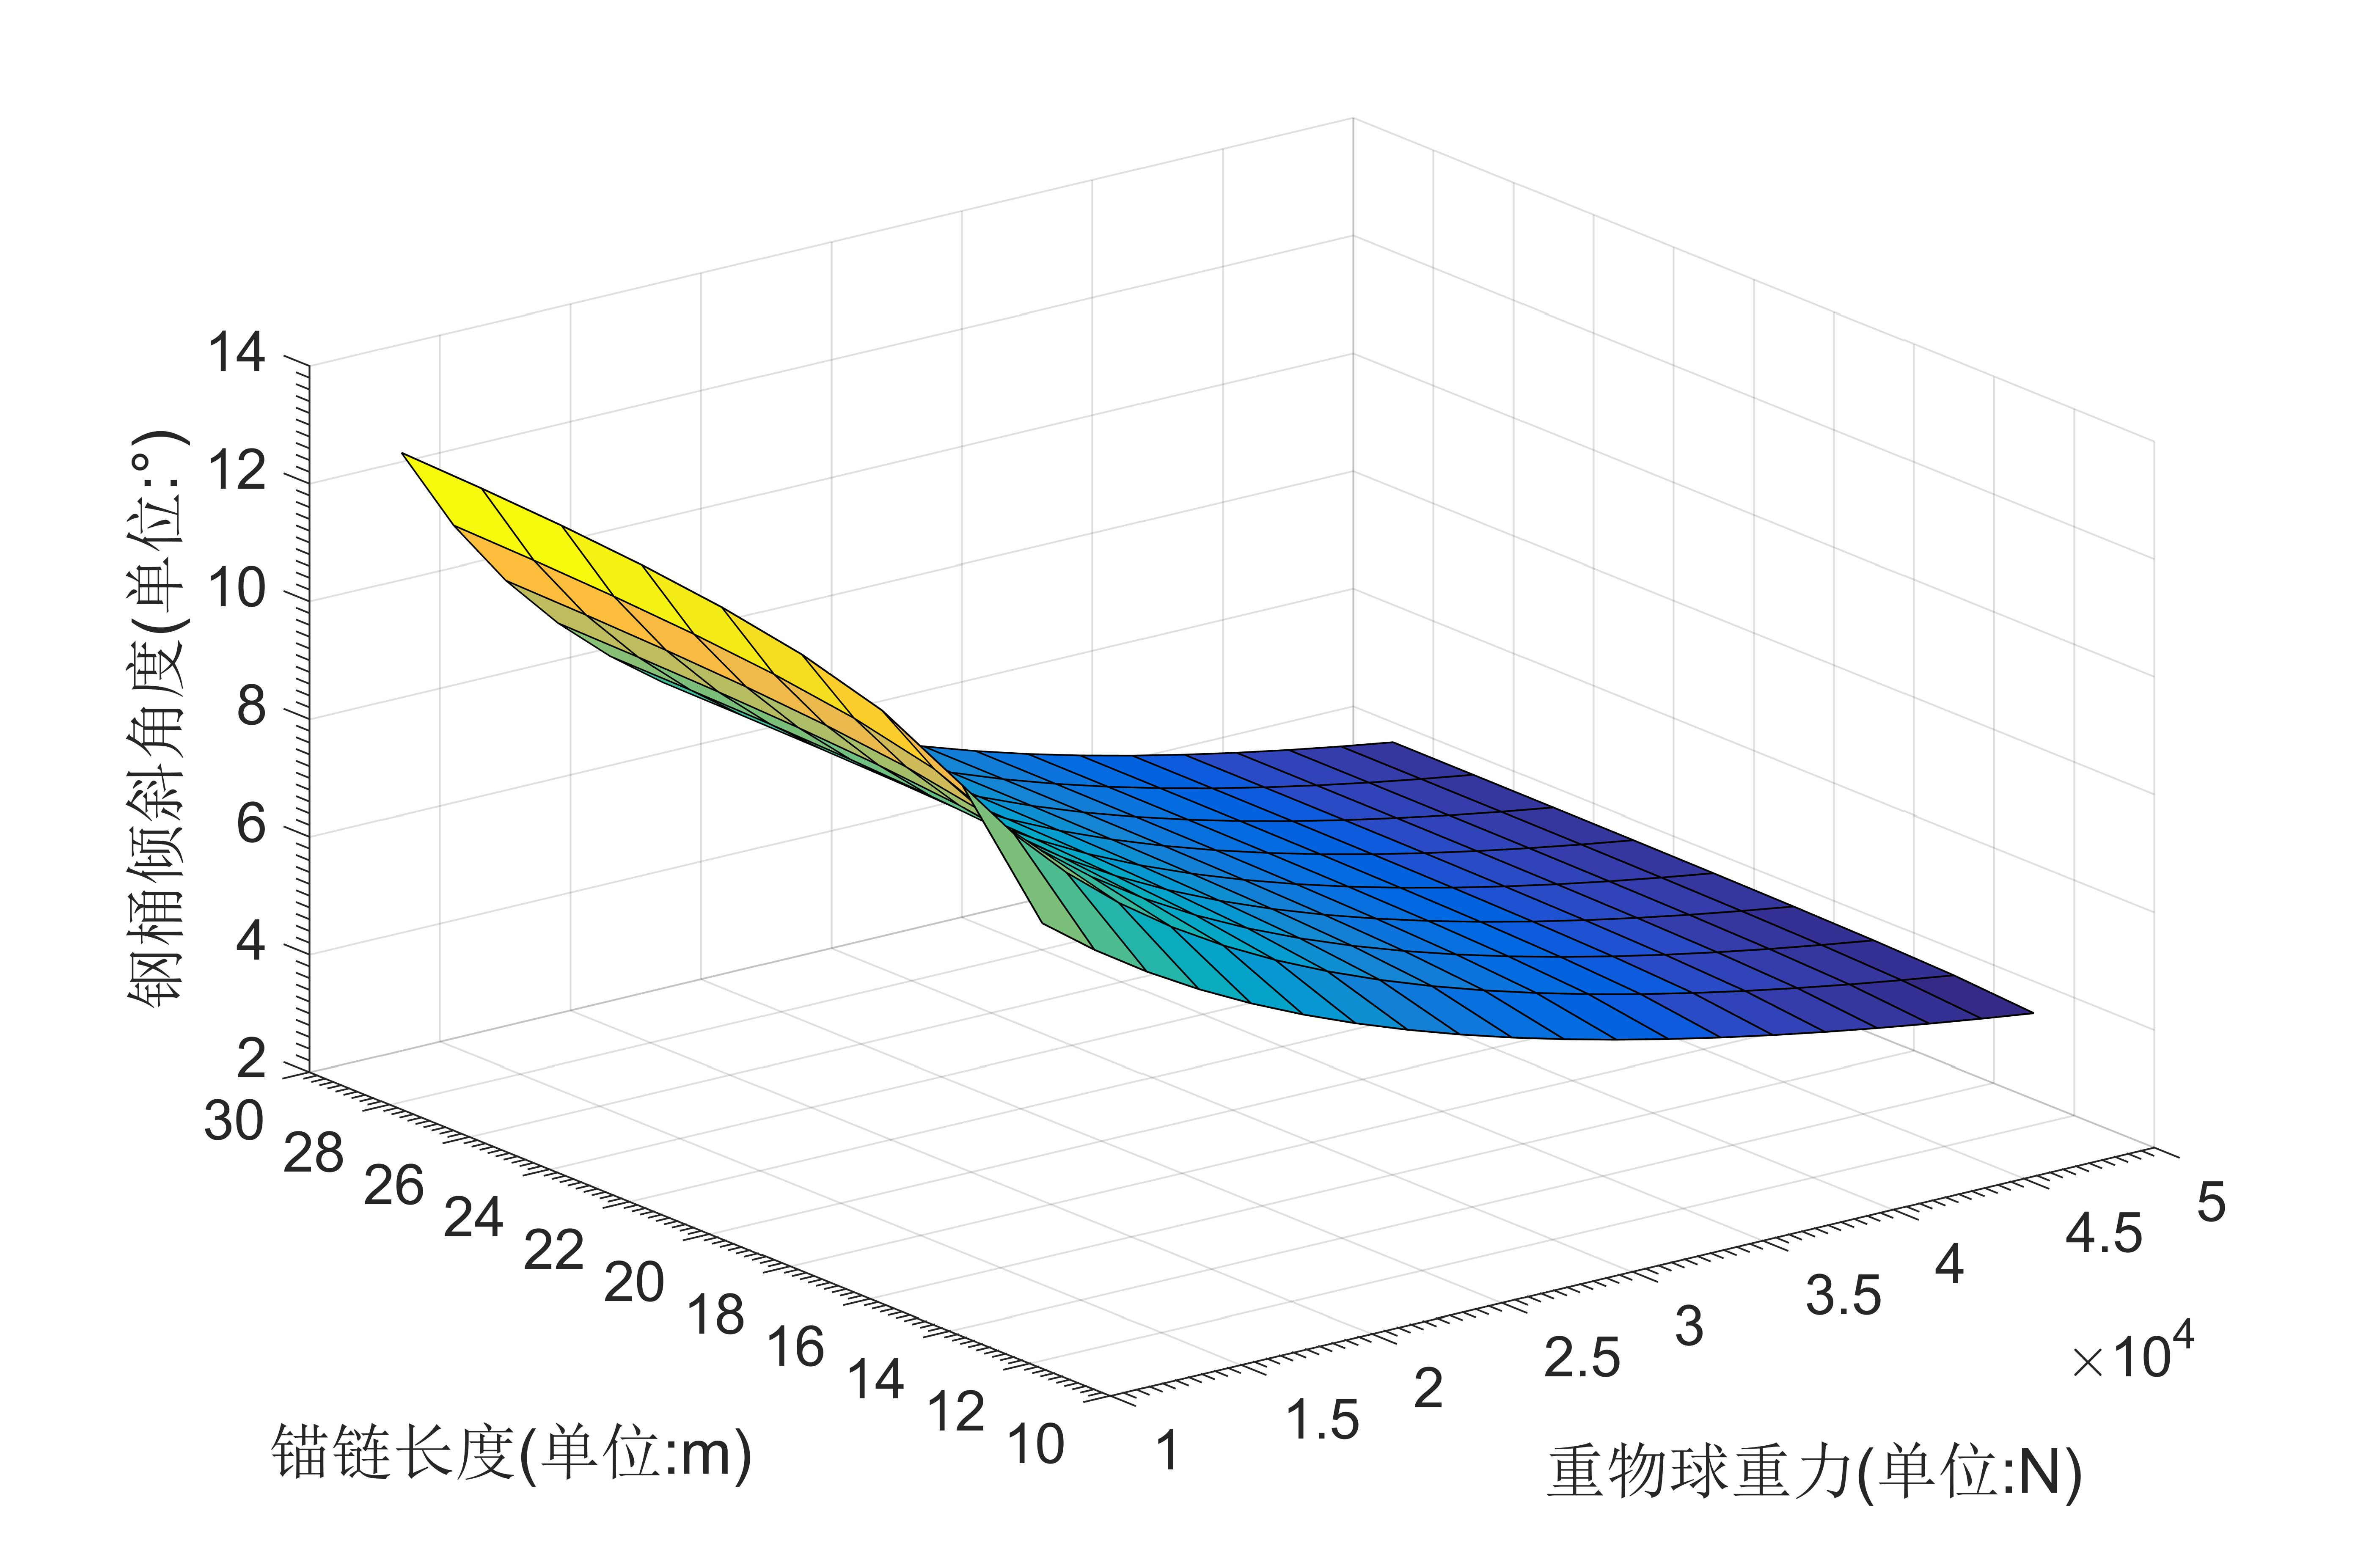
\includegraphics[width=\textwidth]{img/II_18_theta.jpg}   
    \caption{$\theta$变化图}   
    \label{fig:2_18_theta}   
  \end{minipage}
   \begin{minipage}[t]{0.5\linewidth} % 如果一行放2个图,用0.5,如果3个图,用0.33  
      \centering   
      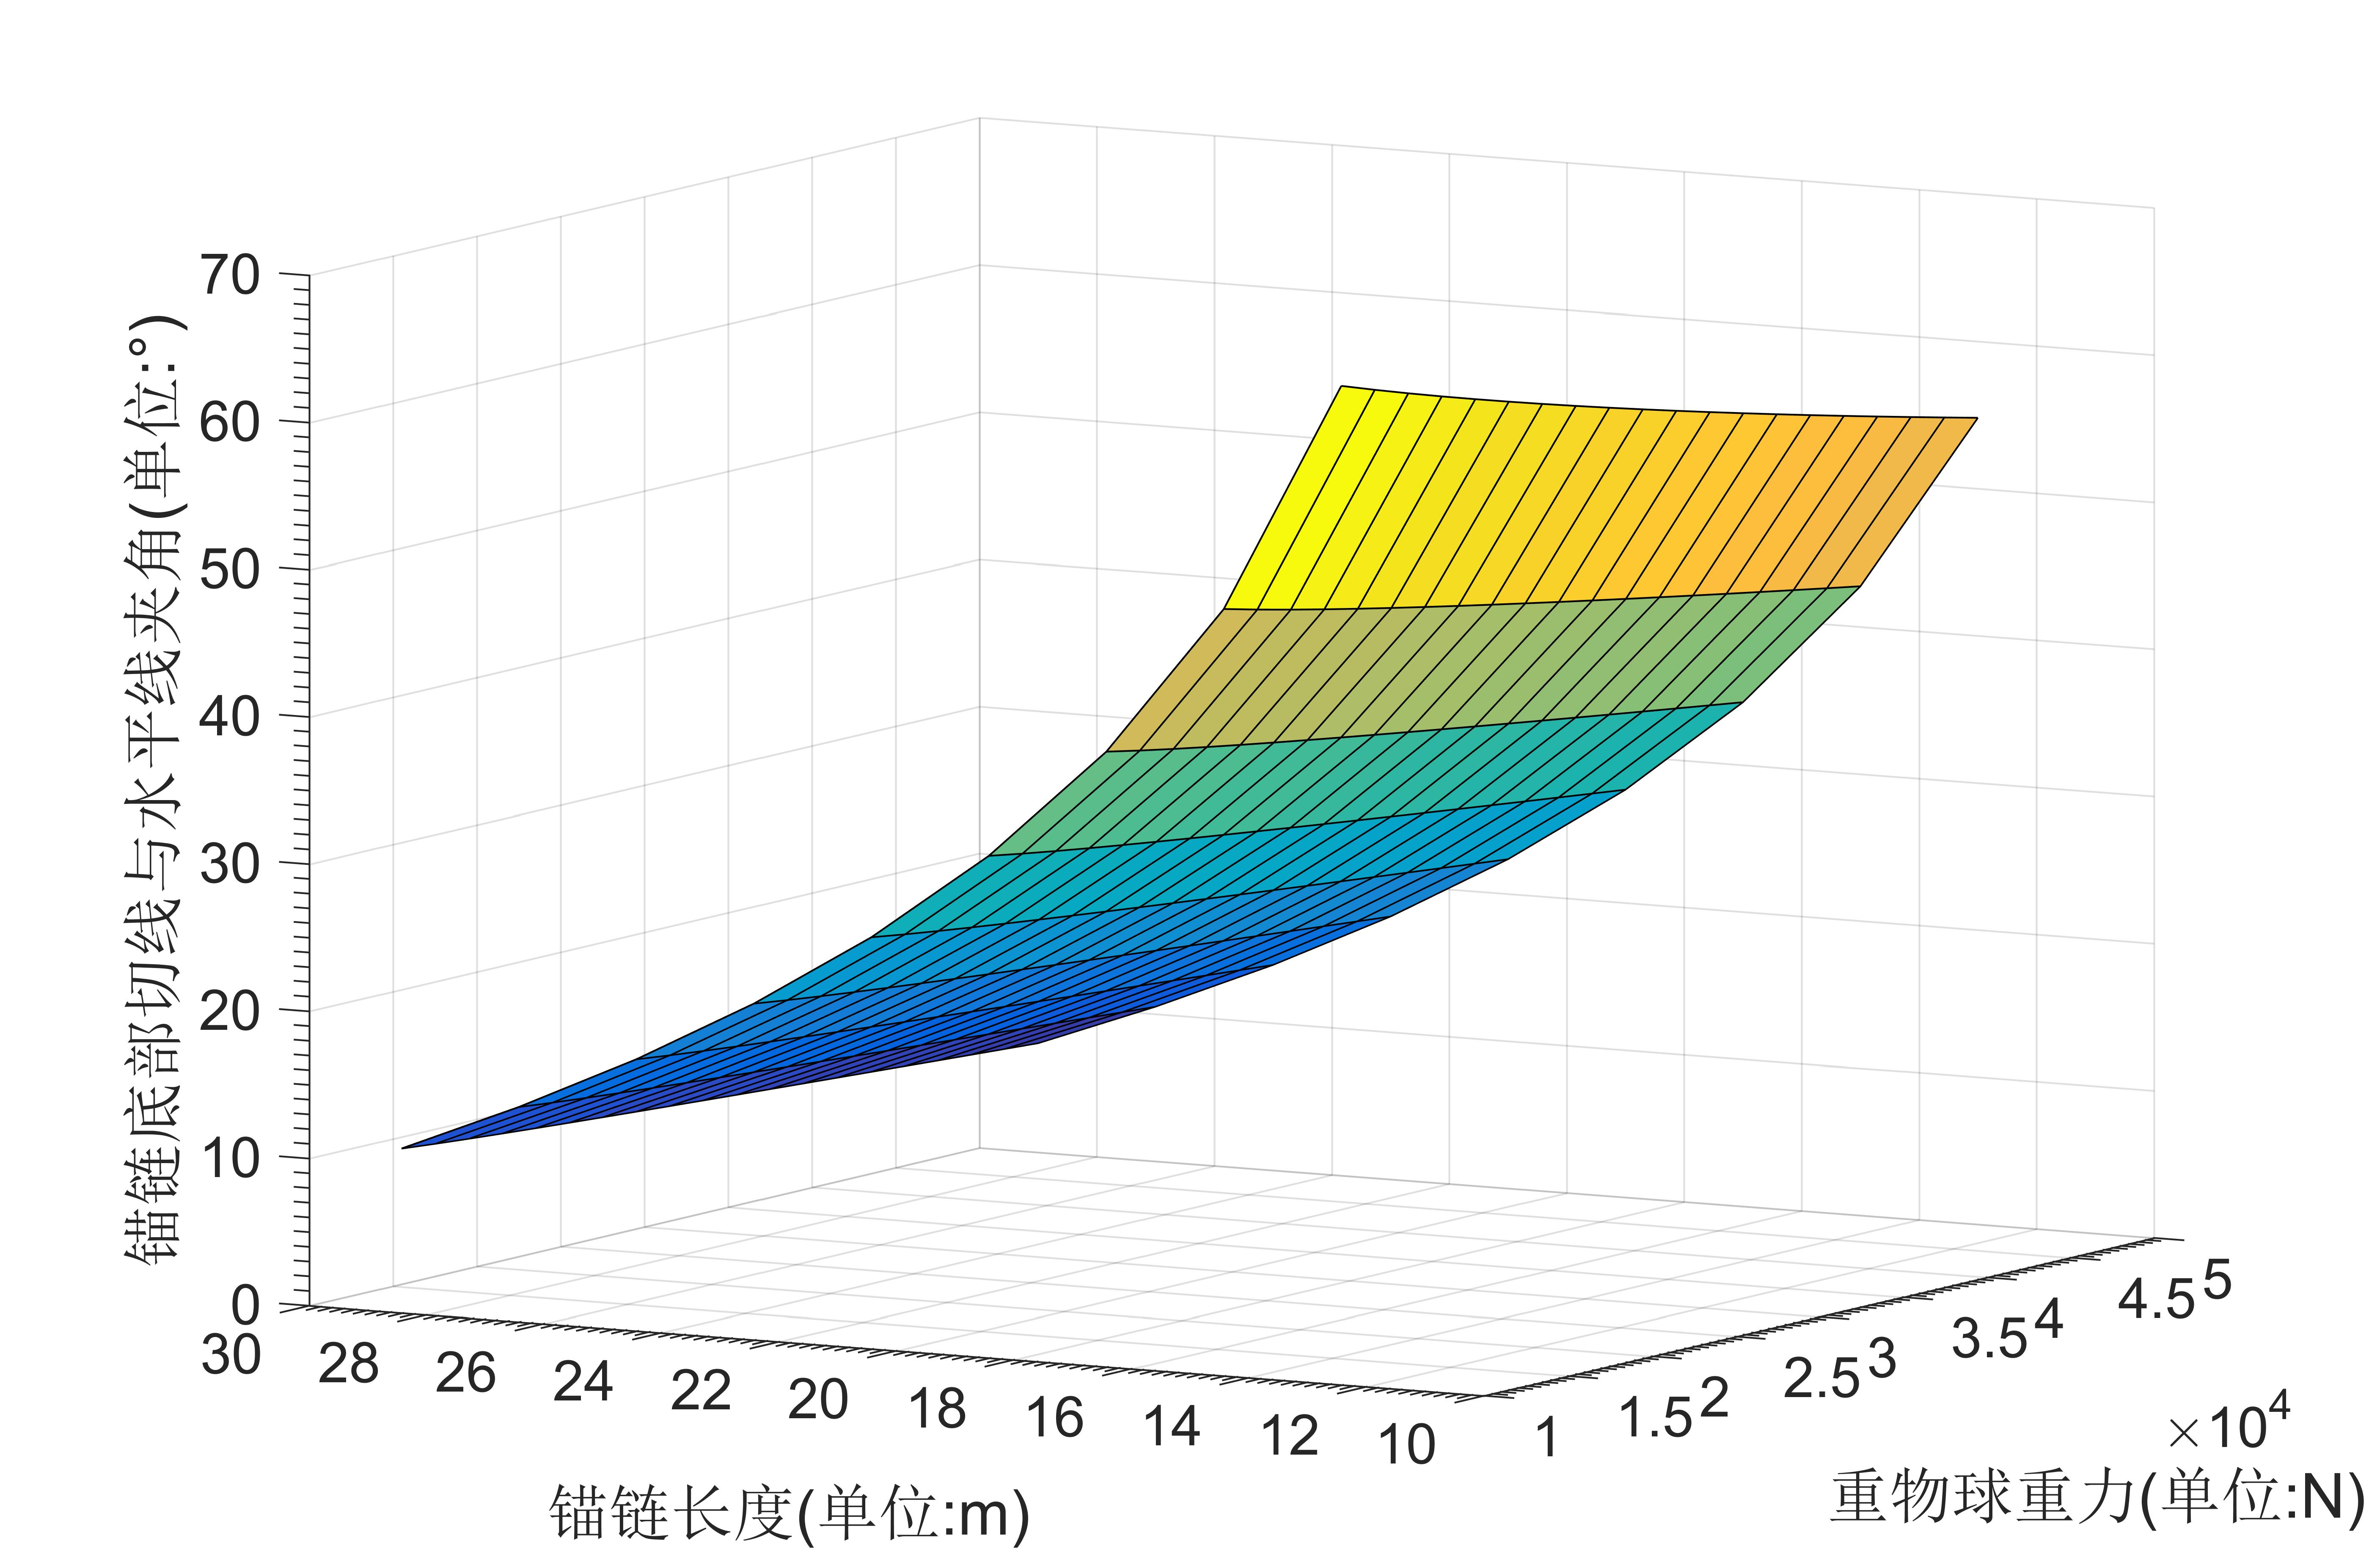
\includegraphics[width=\textwidth]{img/II_18_beta.jpg}   
      \caption{$\beta$变化图}   
      \label{fig:2_18_beta}   
    \end{minipage} 
\end{figure}
\begin{figure}[H]
  \begin{minipage}[t]{0.5\linewidth}   
    \centering   
    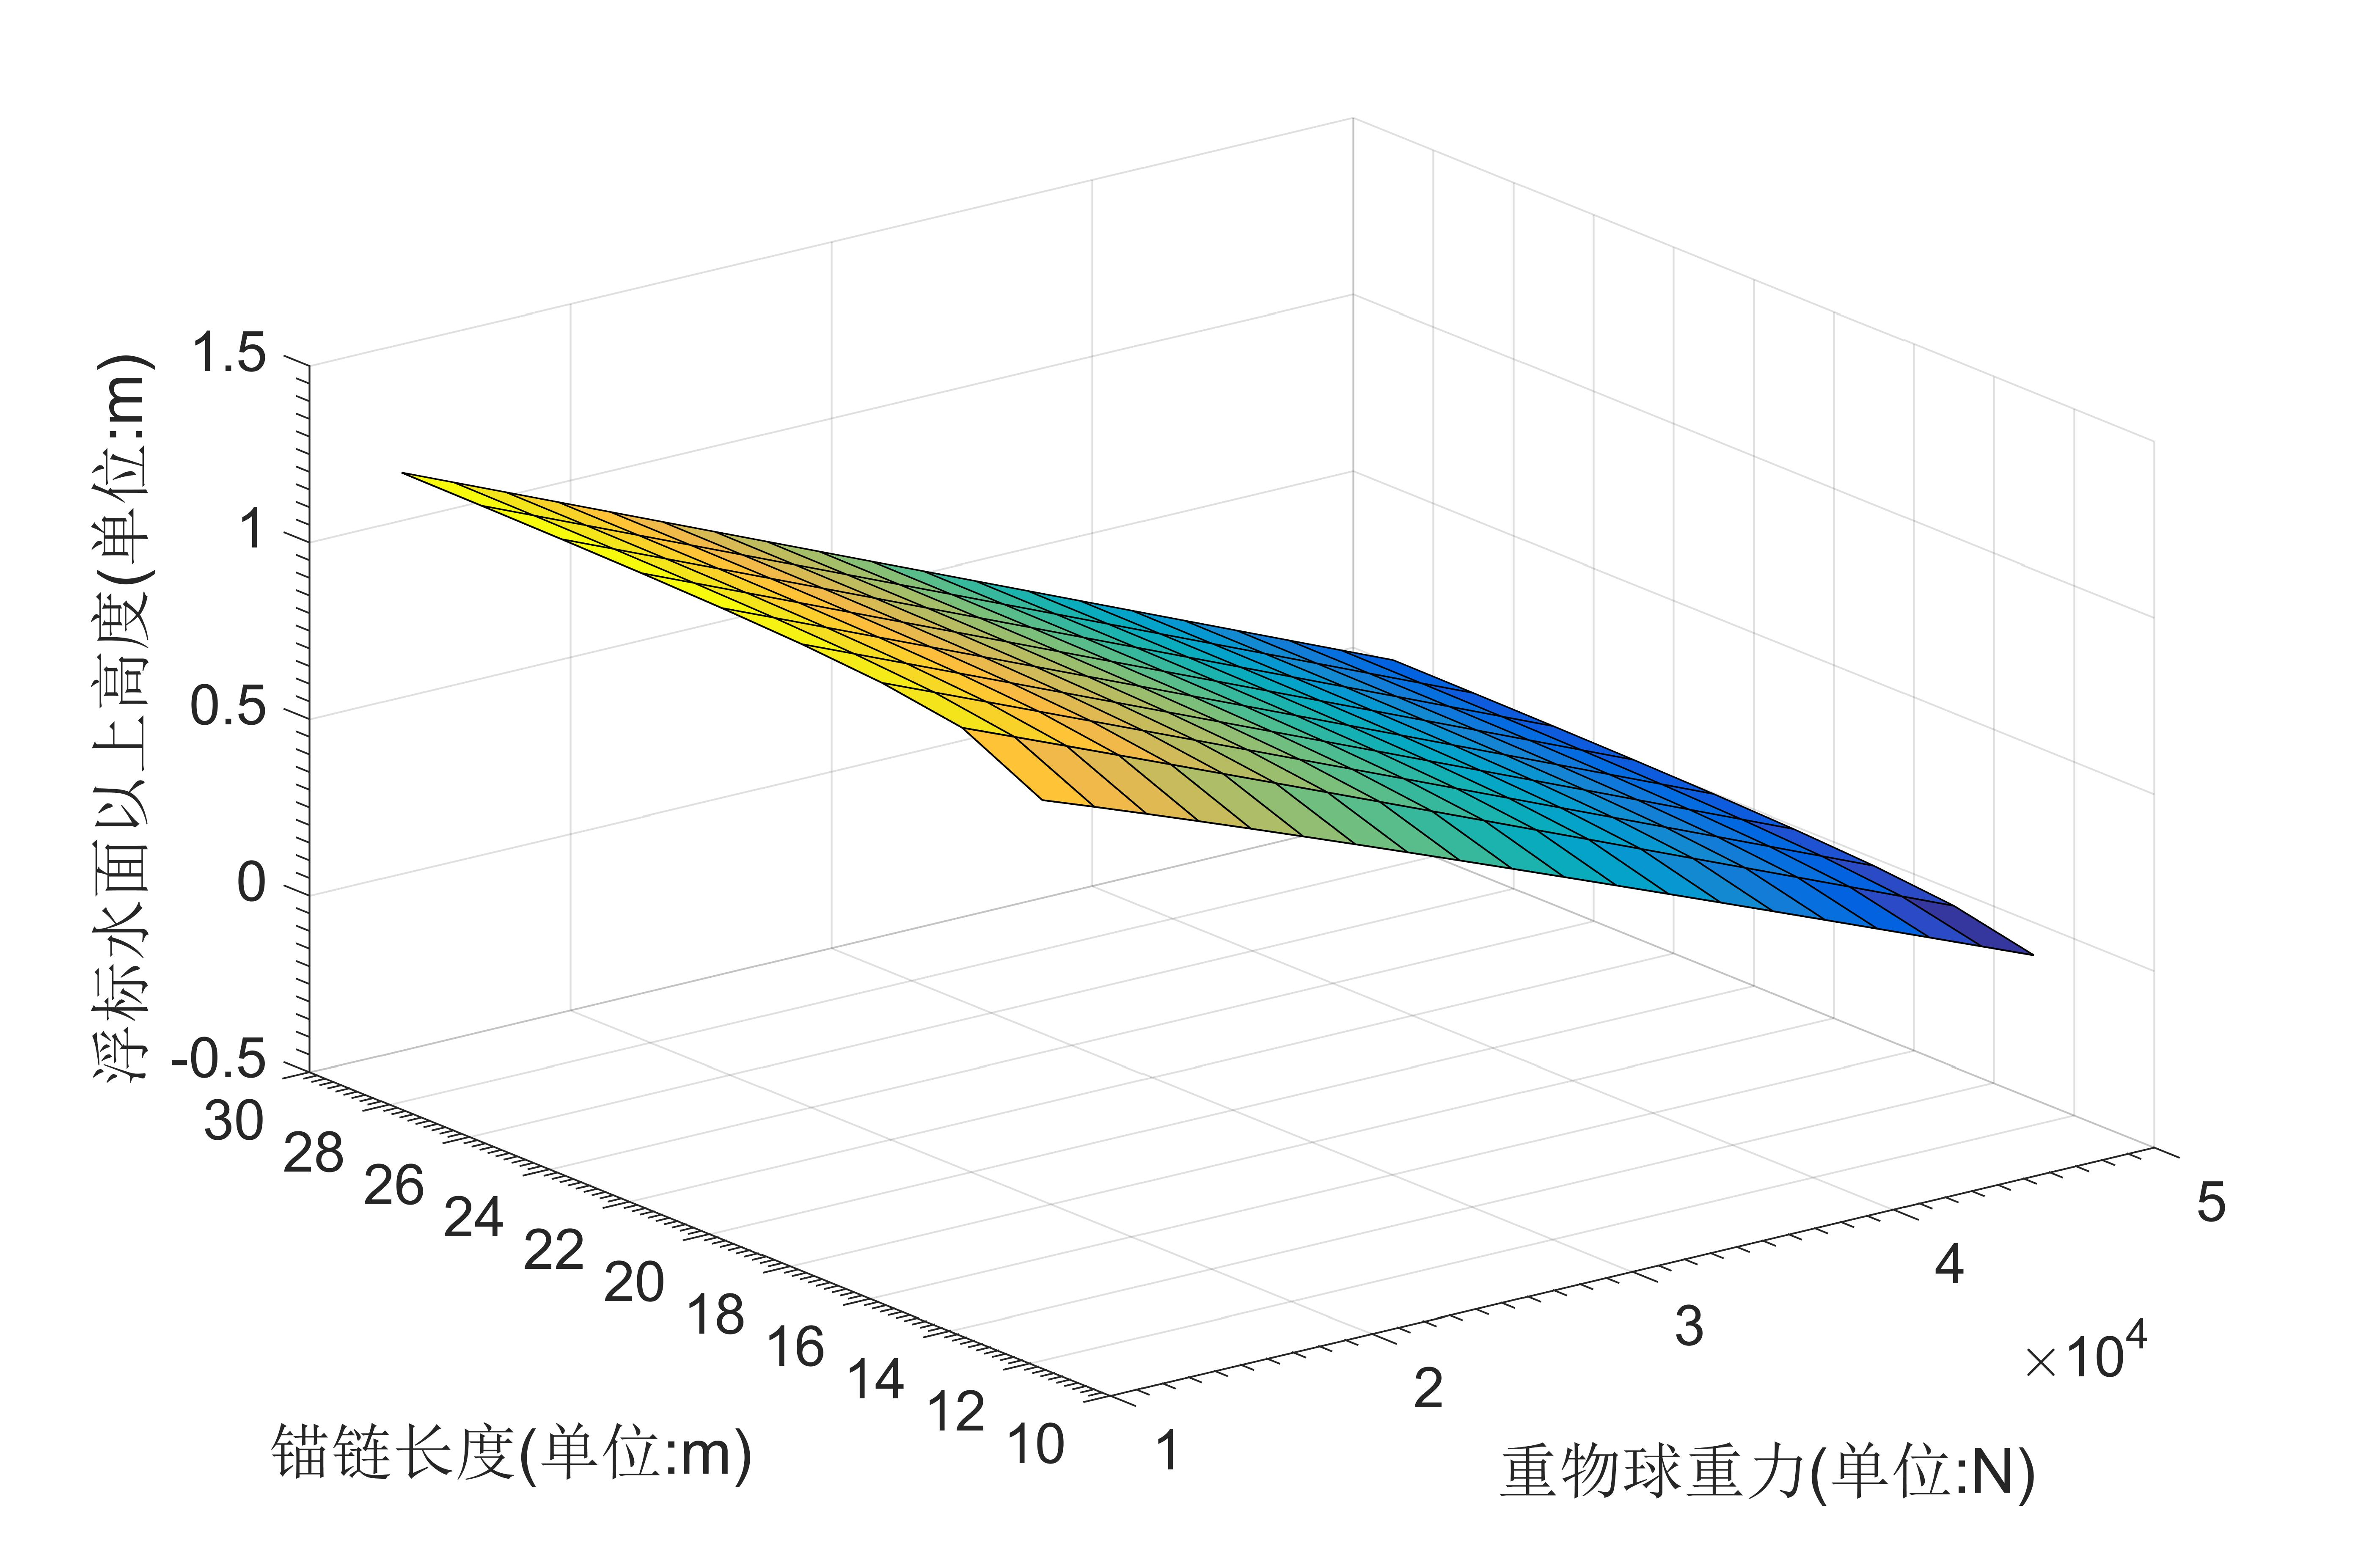
\includegraphics[width=\textwidth]{img/II_18_h.jpg}   
    \caption{$h$变化图}   
    \label{fig:2_18_h}   
  \end{minipage}
   \begin{minipage}[t]{0.5\linewidth} % 如果一行放2个图,用0.5,如果3个图,用0.33  
      \centering   
      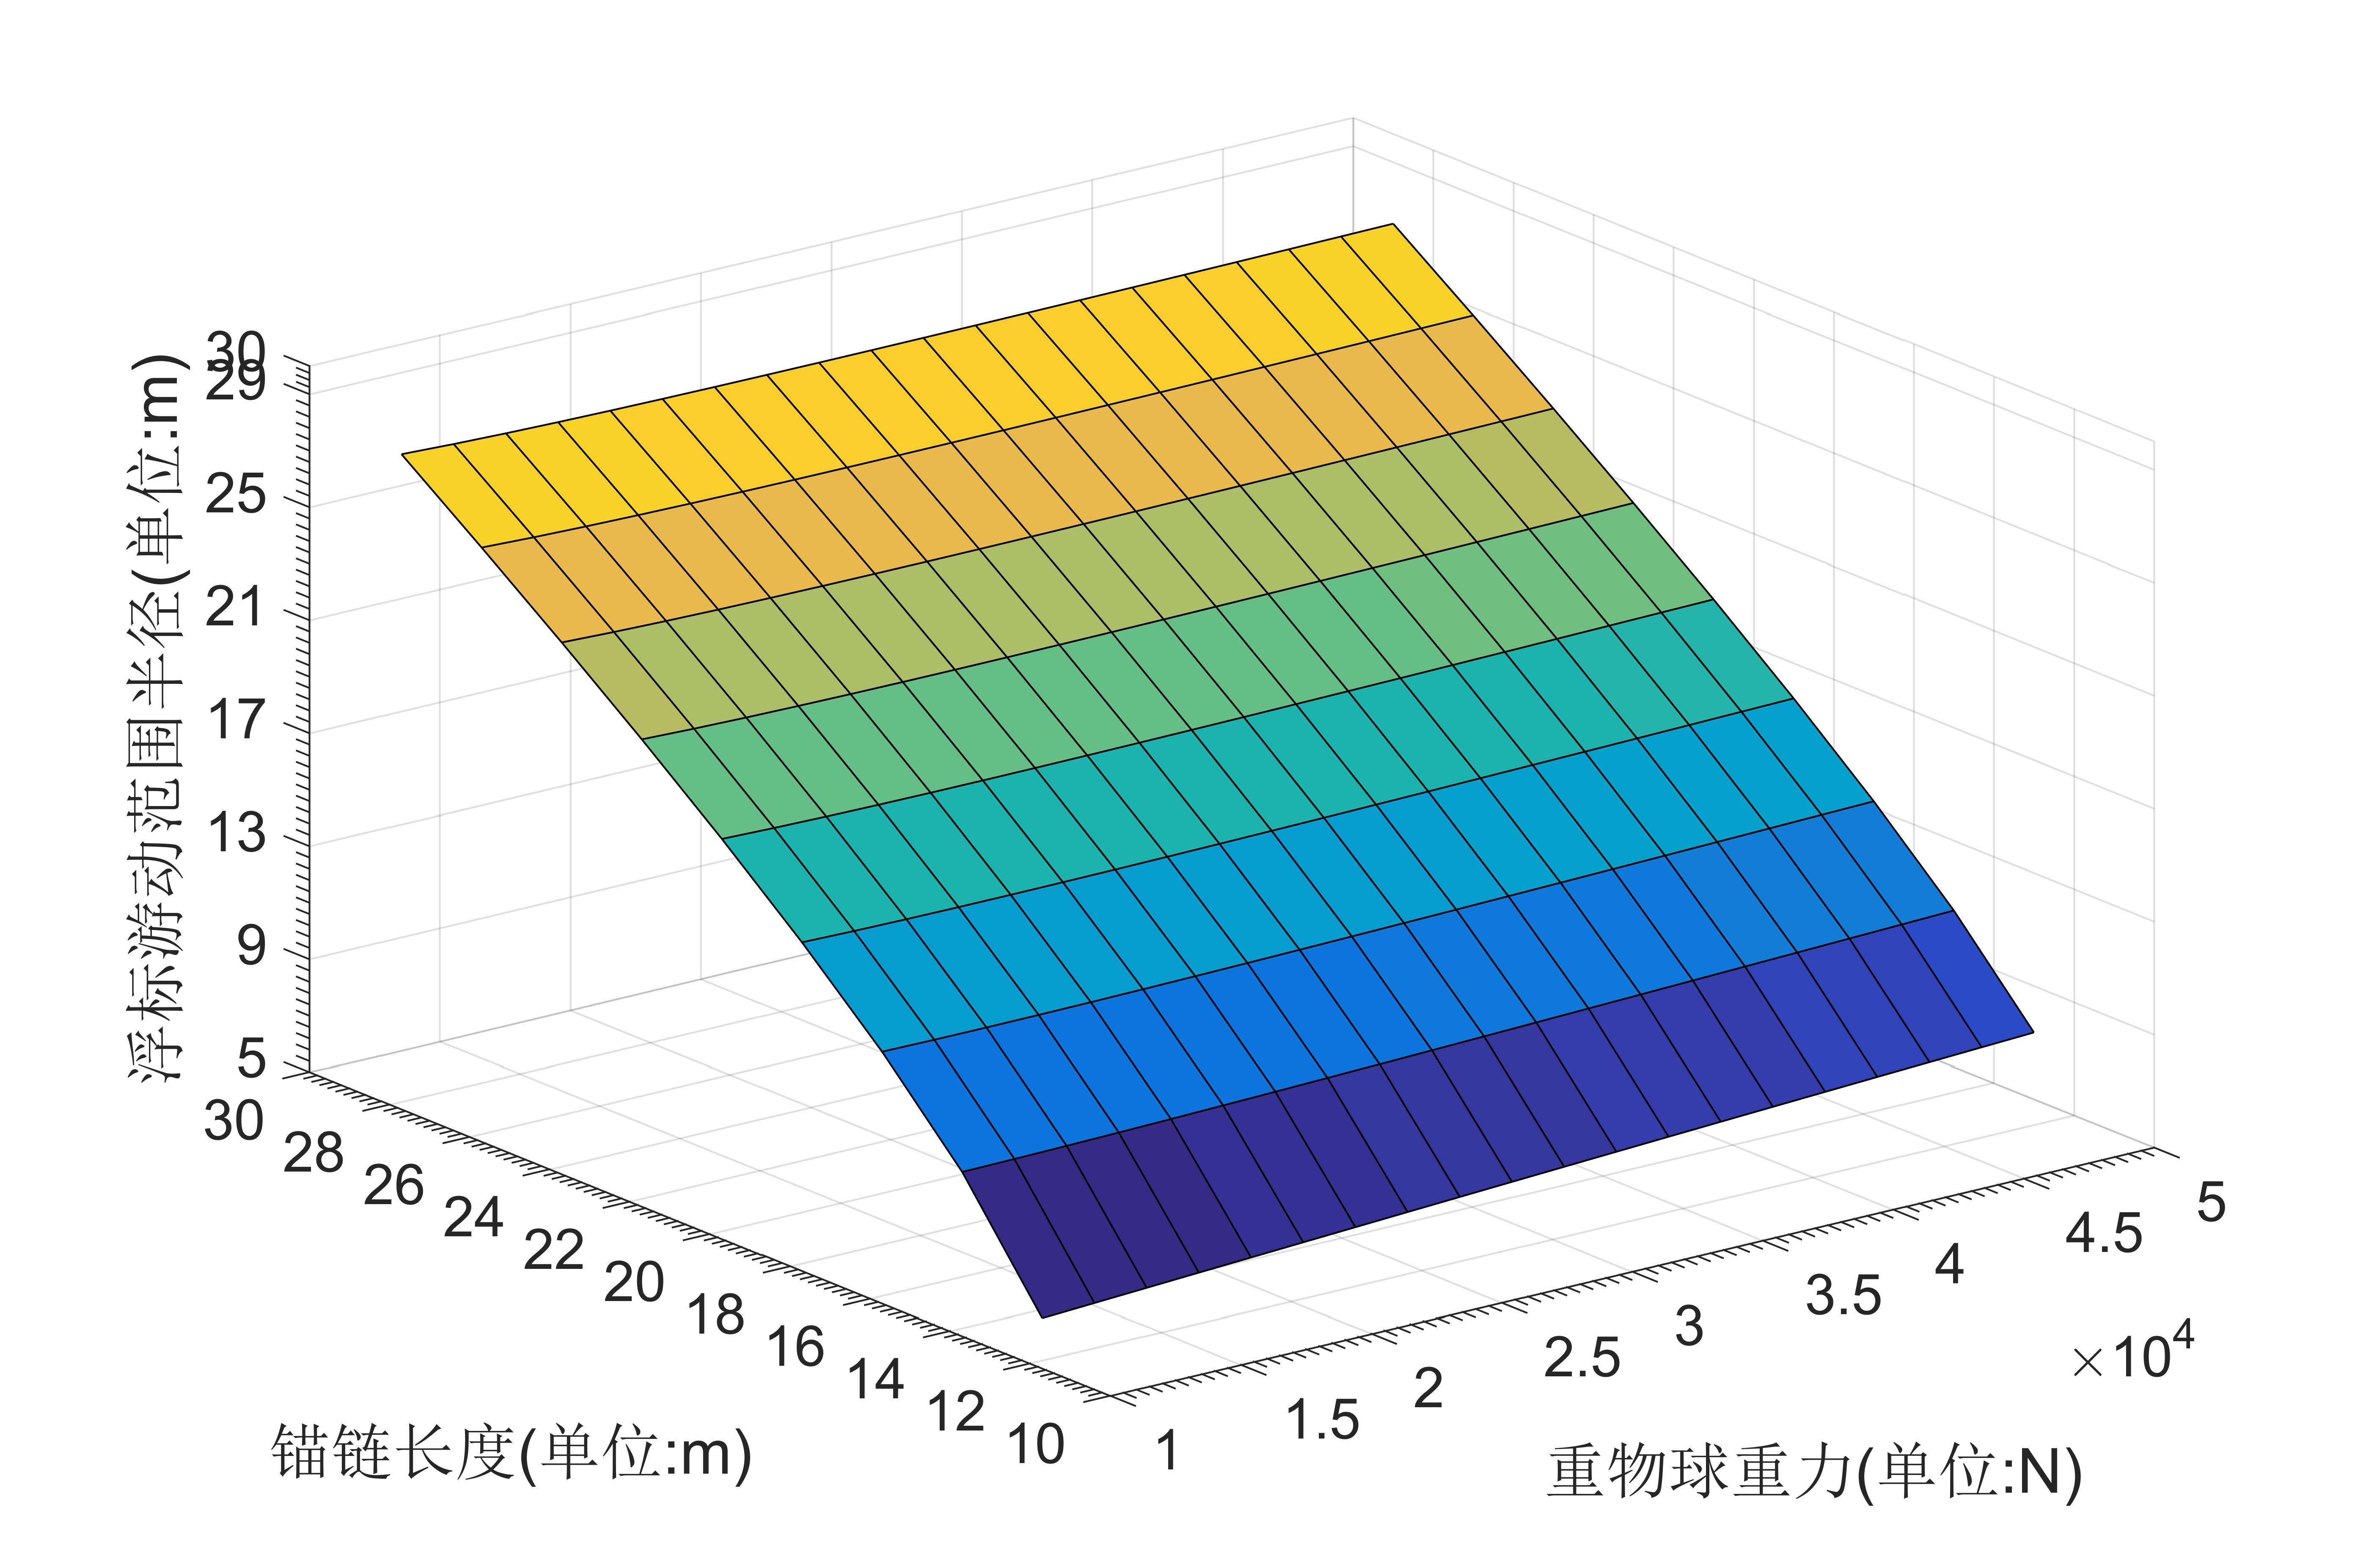
\includegraphics[width=\textwidth]{img/II_18_distance.jpg}   
      \caption{$distance$变化图}   
      \label{fig:2_18_distance}   
    \end{minipage} 
\end{figure}
记重物球重力为$x$轴,锚链长度为$y$轴,各变化量为$z$轴,且正向均为增大的方向。\textbf{可行域}为满足限定条件$\theta\le 5,\beta\le 16$ 的区域。\par 
简单地观察各图易知,每个图总会在$x$方向或$y$方向变化不大,而几乎仅仅受某一变量的影响。这就导致我们可以简单地确定可行解域的大体位置,如图\ref{fig:2_18_theta}中,由$\theta\le 5$条件限制的可行解域即为整个遍历范围的右侧一部分;如图\ref{fig:2_18_theta}中,由$\beta\le 16$条件限制的可行解域即为整个遍历范围的上侧一部分。(此处以x轴正方向为右,y轴正方向为上)两者交叉即得可行解域大致为整个遍历范围的右上角一部分。我们可以通过绘制等高线的方法直观地将这片区域表示出来,如图\ref{fig:II_7_contour1}所示:\par
 \begin{figure}[H]
 	\centering
 	\includegraphics*[width=0.8\textwidth]{img/II_7_contour1}
 	\caption{关于钢桶倾斜角和锚链底端切线水平夹角的双重等高线图}
 	\label{fig:II_7_contour1}
 \end{figure}
从图中可以看到$\theta =5$的等高线变化幅度不是很大,$\beta =16$的等高线有一定倾斜度,因此我们把可能最优解域定为两等高线交点右侧$\beta$等高线上的点。\par 
进一步分析另外两个目标变量,在可行解域上,$h$可近似认为仅随$x$的减小而增大,\\$distance$可近似认为仅随$y$的减小而减小。因而为了使$distance$尽可能小,可能的最优解一定在可行解域的下部边界上。\par 
再考虑边界上的最优解。由于$\theta $与$h$关于$x$的变化方向相反,而两者又都是需要优化的量,故必须确定一个新的目标量将这两者综合起来考虑。题目中没有给出两者的权重分配如何,我们采用赋权值的多目标规划模型\cite{mathmodel},转化为单一目标规划,目标函数定义如式\ref{target_function}:
\begin{equation}
	V_{target} = \frac{1}{2}\cdot (\frac{\theta}{5}+\frac{2-h}{2})
	\label{target_function}
\end{equation}
综上所述,对于某一个特定条件,即水深、锚链型号固定的情况,寻找其锚链长度和重物球重量的最优解的算法如下:\par 
\begin{enumerate}
	\item 遍历两个变量的所有合理值,作出两条等高线
	\item 用两条等高线的数据线性拟合为两个直线方程,用这两个方程求出两条等高线的交点。
	\item 遍历交点右侧$\beta$等高线的目标函数\ref{target_function}值,作出下凸函数图像,求出最小值点的横纵坐标,即为最优解。
\end{enumerate}
现在我们考虑不同锚链型号和不同水深对最优解以及最优解条件下游动区域的影响,使用以上算法求出数据如下:
\begin{table}[!htp]
	\centering
	\caption{重物球重力$(\times10^4N)$}
	\label{table:gravity}
	\centering
	\begin{tabular*}{0.55\textwidth}{c|ccc}
		\hline
		\diagbox[dir=SE]{锚链型号}{水深$m$} & 16 & 18 & 20 \\
		\hline
		\uppercase\expandafter{\romannumeral1} & 4.6410 & 4.6357 & 4.6324\\
		\uppercase\expandafter{\romannumeral2} & 4.6207 & 4.5361 & 4.5305\\
		\uppercase\expandafter{\romannumeral3} & 4.5163 & 4.5065 & 4.4238\\
		\uppercase\expandafter{\romannumeral4} & 4.3991 & 4.3831 & 4.3712\\
		\uppercase\expandafter{\romannumeral5} & 4.3671 & 4.2529 & 4.2283\\
		\hline
	\end{tabular*}
\end{table}
\begin{table}[H]
	\centering
	\caption{锚链长度 $(m)$ }
	\label{table:chain_length}
	\centering
	\begin{tabular*}{0.51\textwidth}{c|ccc}
		\hline
		\diagbox[dir=SE]{锚链型号}{水深$m$} & 16 & 18 & 20 \\
		\hline
		\uppercase\expandafter{\romannumeral1} & 24.67 & 28.90 & 32.91\\
		\uppercase\expandafter{\romannumeral2} & 20.77 & 24.16 & 27.33\\
		\uppercase\expandafter{\romannumeral3} & 17.98 & 20.80 & 23.54\\
		\uppercase\expandafter{\romannumeral4} & 16.05 & 18.59 & 21.01\\
		\uppercase\expandafter{\romannumeral5} & 14.61 & 16.99 & 19.26\\
		\hline
	\end{tabular*}
\end{table}
\begin{table}[H]
	\centering
	\caption{评价函数}
	\label{table:judge_function}
	\centering
	\begin{tabular*}{0.62\textwidth}{c|ccc}
		\hline
		\diagbox[dir=SE]{锚链型号}{水深$m$} & 16 & 18 & 20 \\
		\hline
		\uppercase\expandafter{\romannumeral1} & 0.861395 & 0.861392 & 0.861391\\
		\uppercase\expandafter{\romannumeral2} & 0.861404 & 0.861408 & 0.861395\\
		\uppercase\expandafter{\romannumeral3} & 0.861391 & 0.861402 & 0.861399\\
		\uppercase\expandafter{\romannumeral4} & 0.861405 & 0.861391 & 0.861414\\
		\uppercase\expandafter{\romannumeral5} & 0.861410 & 0.861394 & 0.861401\\
		\hline
	\end{tabular*}
\end{table}
\begin{table}[H]
	\centering
	\caption{游动半径$(m)$}
	\label{table:distance}
	\centering
	\begin{tabular*}{0.5\textwidth}{c|ccc}
		\hline
		\diagbox[dir=SE]{锚链型号}{水深$m$} & 16 & 18 & 20 \\
		\hline
		\uppercase\expandafter{\romannumeral1} & 23.21 & 26.94 & 30.41\\
		\uppercase\expandafter{\romannumeral2} & 18.89 & 21.61 & 24.06\\
		\uppercase\expandafter{\romannumeral3} & 15.62 & 17.62 & 19.48\\
		\uppercase\expandafter{\romannumeral4} & 13.25 & 14.80 & 16.20\\
		\uppercase\expandafter{\romannumeral5} & 11.35 & 12.63 & 13.74\\
		\hline
	\end{tabular*}
\end{table}
分析表\ref{table:gravity}、表\ref{table:chain_length}、表\ref{table:judge_function}和表\ref{table:distance}中的数据得出以下结论:
\begin{enumerate}
	\item 水深增大,重物球重力和锚链长度都在增大,又因为若想满足两个角度限制的条件,必须选择最大的重物球重力和最长的锚链长度。故对于每个锚链型号,都应选择水深20米时的结果。
	\item 相同水深情况下,锚链密度越大,游动半径越小。
	\item 不管水深和锚链型号为多少,评价函数的值几乎没有差别。
	\item 综合以上两点考虑,最终得出的最优解为长度为19.26米的V型锚链和重力为$42283N$的重物球。
\end{enumerate}
外部条件为风速$36m/s$,水速为$1.5m/s$,水深为$20m$的情况下,求出的各项数据结果如表\ref{table:result_3}和表\ref{table:pipe_angle_3}所示:
\begin{table}[!htp]
	\centering
	\caption{问题三部分计算结果}\label{table:result_3}
	\centering
	\begin{tabular*}{0.8\textwidth}{ccccc}
		\hline
		风速$(m/s)$ & 钢桶倾斜角$(^\circ)$ & 吃水深度$(m)$ & 游动半径$(m)$ & 锚链参数$a$ \\
		\hline
		36 & 4.1441 & 1.7911 & 14.3234 & 48.8752\\
		\hline
	\end{tabular*}
\end{table}
\begin{table}[H]
	\centering
	\caption{问题一钢管倾斜角计算结果}
	\label{table:pipe_angle_3}
	\begin{tabular*}{0.82\textwidth}{ccccc}
		\hline
		风速$(m/s)$ & 钢桶倾斜角1 & 钢桶倾斜角2 & 钢桶倾斜角3 & 钢桶倾斜角4\\
		\hline
		36 & 0.99743 & 0.99742 & 0.99741 & 0.99740\\
		\hline
	\end{tabular*}
\end{table}

\section{模型总结}

\subsection{模型优点}

\begin{enumerate}

\item 由于本模型通过求解物理力学方程以及悬链线方程得到解,只需输入外部条件参数和锚链型号即可给出需要的重物球重量和锚链长度。对于问题一类型的问题可以快速求解。

\item 当一个参数不确定时,可以通过二分法求解出其范围,得到最优解。对于问题二类型的问题也可以快速地得到解决。

\item 对于问题三,本模型采用基于加权系数法和优先等级法的多目标规划模型,逐步排除了某些自变量对某些维度的影响,并且将某些目标量合并为一种目标量,极大降低了模型复杂度,提高了求解速度。

\end{enumerate}

\subsection{模型缺点}

\begin{enumerate}
\item 本模型建立在优先等级法之上,这种方法本身可能会导致模型落入局部最优解。
\item 对于加权系数法的权值设定过于简单,没有考虑真正的实际情况,而直接做相同比重处理。这样会可能导致对某一要素的优化程度过低。
\item 模型中使用拟合曲线对数据进行拟合时可能输入数据范围太小,或应该使用高次多项式拟合和非线性拟合,以达到更好地效果。
\end{enumerate}


\bibliographystyle{plain}
\bibliography{ref}

\newpage
\appendix
\textbf{附录}
\section{模型求解代码}

\begin{lstlisting}
	% 下标指定:
	% fl 浮标
	% p 钢管
	% b 钢桶
	% s 重物球
	% c 锚链
	format short;
	syms h;% 浮标露出水面高度
	v = 24;% 第一题风速
	u = 1.5;
	d_fl = 2;% 浮标底面直径
	g = 9.8;% 重力加速度
	rho = 1025;% 海水密度
	H = 2;% 浮标高度
	Fw = 0.625*v^2*d_fl*h;% + 374*u^2*d_fl*(H-h);% 水力+风力
	f_fl = rho*g*(H-h)*d_fl^2*pi/4;% 浮力
	G_fl = 1000*g;% 浮标重力
	T(1,:) = [Fw,f_fl-G_fl];% 第一个结点的受力
	% 钢管
	G_p = 10*g;% 钢管重力
	f_p = (1*0.05^2*pi/4)*rho*g;% 钢管浮力
	% T表示六个结点处的受力,其中T(1)到T(5)有递推关系如下:
	for i = 2:5
	    T(i,:) = [T(i-1,1),T(i-1,2)-G_p+f_p];
	end
	% 钢桶
	G_s = 1200*g;% 重物球重力
	f_b = (0.3^2*pi/4)*1*rho*g;% 钢桶浮力
	G_b = 100*g;% 钢桶重力
	% 第六个结点
	T(6,:) = [T(5,1),T(5,2)+f_b-G_b-G_s];% 锚链上端结点受力
	% 锚链上方高度
	for i=1:4
	    temp = (T(i+1,1)+T(i,1))/(T(i+1,2)+T(i,2));
	    t(i) = sqrt(1/(1+temp^2));% t(1~4)为每根钢管倾斜角度的余弦值
	    k(i) = sqrt(temp^2/(1+temp^2));
	end
	temp = (T(6,1)+T(5,1))/(T(5,2)+T(6,2)+G_s);% 钢桶倾斜角度的正切值
	length = sum(t) + sqrt(1/(1+temp^2));% 锚链上方高度
	length2 = sum(k)+sqrt(temp^2/(1+temp^2));%x方向长度投影

	% 锚链
	w = 7*g;%单位长度锚链重力
	R = T(6,1);% 水平方向受力
	L = 22.05;% 锚链长度
	a = R/w;% 悬链线方程参数
	% 以锚链底端为原点,水平方向为横轴,竖直方向为纵轴建立平面直角坐标系
	% 考虑没有铺底的情况
	syms x;% 第六个结点的横坐标
	% 铺底的方法
	x1 = solve(sinh(x/a)==T(6,2)/T(6,1),x);% 将x以h表示
	y1 = a*cosh(x1/a)-a;% 求出第六个结点的纵坐标
	L_right = a*sinh(x1/a);
	% 解方程
	fun1 = matlabFunction(length+y1(1)+H-h-18);
	[hres1,fval1,exitflag1] = fsolve(fun1,1);
	fun2 = matlabFunction(length+y1(2)+H-h-18);
	[hres2,fval2,exitflag2] = fsolve(fun2,1);
	% 通过检验exitflag值,决定哪一个方程有解
	% 判断哪个是解
	if exitflag1<0
	    hres = hres2;
	    flag = 2;
	else
	    hres = hres1;
	    flag = 1;
	end
	L_right = eval(subs(L_right,h,hres));
	if L > L_right
	    %铺底的情况
	    yres = eval(subs(y1(flag),h,hres));% 第六个节点高度
	    L_right = eval(subs(L_right(flag),h,hres));% 锚链在水平线上方的长度
	    x1 = eval(subs(x1(flag),h,hres));% 锚链水平方向长度
	    length2 = eval(subs(length2,h,hres));% 第六个节点上方水平方向长度
	    distance = L-L_right+length2+x1; %水平偏移
	    theta = eval(subs(atan(temp)*180/pi,h,hres));% 钢桶倾斜角度
	    pipetheta = eval(subs(acos(t)*180/pi,h,hres));% 钢管倾斜角度
	    a = eval(subs(a,h,hres));
	    theta
	    pipetheta
	    x1
	    yres
	    hres
	    distance
	else
	    % 不铺底的情况
	    beta = (T(6,2)-w*L)/T(6,1);% 锚链低端切线斜率
	    x2 = solve(beta*cosh(x/a) + sinh(x/a)*(beta^2 + 1)^(1/2)==T(6,2)/T(6,1),x);% 将x以h表示
	    y2 = a*beta*sinh(x2/a) + a*cosh(x2/a)*(beta^2 + 1)^(1/2)-a*sqrt(beta.^2+1);% 求出第六个结点的纵坐标
	    fun1 = matlabFunction(length+y2(1)+H-h-18);
	    hres1 = fsolve(fun1,1.2);
	    fun2 = matlabFunction(length+y2(2)+H-h-18);
	    hres2 = fsolve(fun2,1.2);
	    if isreal(hres1)
	        hres = hres1;
	        flag = 1;
	    else
	        hres = hres2;
	        flag = 2;
	    end
	    betatemp = eval(subs(beta,h,hres));
	    betares = atan(betatemp)*180/pi;% 锚链底部切线与水平线夹角
	    x2 = eval(subs(x2(flag),h,hres));% 第六个结点横坐标
	    length2 = eval(subs(length2,h,hres));% 第六个节点上方水平方向长度
	    distance = length2+x2; %水平偏移
	    theta = eval(subs(atan(temp)*180/pi,h,hres));% 钢桶倾斜角度
	    yres = eval(subs(y2(flag),h,hres));% 第六个节点纵坐标
	    pipetheta = eval(subs(acos(t)*180/pi,h,hres));% 四个钢管的倾斜角
	    a = eval(subs(a,h,hres));% 悬链线参数
	    theta
	    pipetheta
	    x2
	    yres
	    hres
	    a
	    pipetheta
	    betatemp
	    betares
	end
\end{lstlisting}

\section{二分法搜索代码}
\begin{lstlisting}
% 对指定参数进行二分法搜索
function result = qsearch()
	result=zeros(20,3);
    left = 2500*9.8;right = 3500*9.8;
    % 迭代次数为20
	for i = 1:20
        x = (left+right)/2;
        [a,b]=t2(x);
        result(i,2:3)=[a,b];
        result(i,1)=x/1000;
        if a>0
            left = x;
        else
            right = x;
        end
    end
end
\end{lstlisting}

\section{问题三代码}
\begin{lstlisting}
	clear;clc;
	result = zeros(3,3);
	for depthindex = 1:3
	    m = 20:1:30;mi=size(m);mi=max(mi);
	    n = 30000:1000:40000;ni=size(n);ni=max(ni);
	    H = zeros(mi,ni);
	    D = zeros(mi,ni);
	    T = zeros(mi,ni);
	    B = zeros(mi,ni);
	    for i = 1:mi
	        for j = 1:ni
	            [hres,distance,theta,betares,xres,yres] = t3(m(i),n(j),14+depthindex*2);
	            H(i,j) = hres;
	            D(i,j) = distance;
	            T(i,j) = theta;
	            B(i,j) = betares;
	        end
	    end
	    [x,y] = meshgrid(n,m);
	    figure(depthindex*2-1);
	    v1 = [5,5];
	    [Ct1,ht1] = contour(x,y,T,v1);
	    clabel(Ct1,ht1);
	    x1 = Ct1(1,:);y1 = Ct1(2,:);
	    y1(x1<35000) = [];x1(x1<35000)=[];
	    y1(x1>36000) = [];x1(x1>36000)=[];
	    a = polyfit(x1,y1,1);
	    hold on;
	    v2 = [4,7];
	    [Ct2,ht2] = contour(x,y,T,v2);
	    clabel(Ct2,ht2);
	    v3 = [16,16];
	    [Cb1,hb1] = contour(x,y,B,v3);
	    x2 = Cb1(1,:);y2 = Cb1(2,:);
	    y2(x2<35000) = [];x2(x2<35000)=[];
	    y2(x2>36000) = [];x2(x2>36000)=[];
	    k = polyfit(x2,y2,1);
	    clabel(Cb1,hb1);
	    v4 = [10,22,28];
	    [Cb2,hb2] = contour(x,y,B,v4);
	    clabel(Cb2,hb2);
	    syms t;
	    xres = solve(a(1)*t+a(2)==k(1)*t+k(2),t);
	    xres = max(xres);
	    yres = k(1)*xres+k(2);
	    xres=eval(xres);
	    yres = eval(yres);
	    plot(xres,yres,'.');
	    [hres,distance,theta,betares,x6,y6] = t3(yres,xres,14+depthindex*2);
	    x3 = linspace(xres,50000,20);
	    num = max(size(x3));
	    y3 = k(1)*x3+k(2);
	    evalfunc = zeros(1,num);
	    for j = 1:num
	        [hres,distance,theta,betares,x6,y6] = t3(y3(j),x3(j),14+depthindex*2);
	        evalfunc(j) = (theta/5+(2-hres)/2)/2;
	    end
	    figure(depthindex*2);
	    plot(x3,evalfunc);
	    [val_opt,index] = min(evalfunc);
	    x_opt = x3(index);
	    y_opt = y3(index);
	    result(depthindex,:) = [x_opt,y_opt,val_opt];

	end

	result
\end{lstlisting}

\end{document}